\documentclass[article,preprintnumbers]{revtex4-1}
\usepackage{graphicx,textcomp}
\usepackage{amsmath,amssymb}
\usepackage{tikz}
%\usepackage{mathtools}
%\usepackage{dcolumn}
\usepackage{color}
\usepackage[normalem]{ulem}
%\usepackage{mathrsfs}
\usepackage[T1]{fontenc}
\usepackage{relsize}



\newcommand{\C}[1]{\ensuremath{\mathrm{C}_{#1}}}

\parskip = 4mm plus 2mm minus 2mm
\parindent = 5mm


\newcount\marcnumber
\marcnumber=1\relax
\newcommand{\marc}[1]{
\marginpar{\color{red}{\bf\the\marcnumber}---#1 }
\global\advance\marcnumber by 1}



\begin{document}

\title{PROGRAM FULLERENE (Version 4.0)\\ -- A Program for the Topological Analysis of Fullerenes --\\ USER'S MANUAL}

\begin{figure}[htbp]
	\centering 
	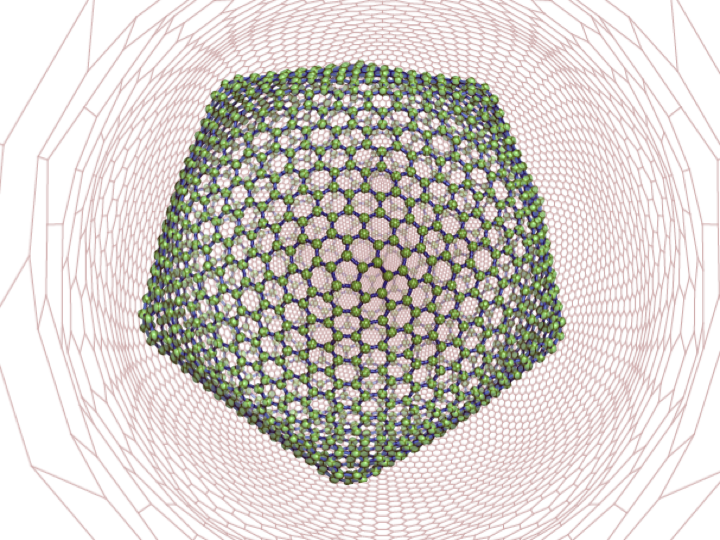
\includegraphics[width=0.6\textwidth]{Toc.png}
    \label{pic:toc}
\end{figure}

\author{Peter Schwerdtfeger}\email[]{p.a.schwerdtfeger@massey.ac.nz}
\author{Lukas Wirz}\email[]{l.wirz@massey.ac.nz}

\affiliation{Center of Theoretical Chemistry and Physics, The New Zealand Institute
for Advanced Study, Massey University Auckland, Private Bag 102904,
North Shore City, 0745 Auckland, New Zealand.}

\author{James Avery}\email[]{avery@nbi.ku.dk}

\affiliation{Niels Bohr Institute, University of Copenhagen, 2100 Copenhagen, Denmark.}
\date{\today}

\maketitle

\clearpage


{\noindent\bf Important Copyright Message:}\\
{\it This is an} {\bf open-source code} {\it and you may use and modify the program at your own will.
If you like to know why, read the article by} Darrel C. Ince1, Leslie Hatton, 
John Graham-Cumming, Nature {\bf 482}, p.485 (2012). {\it However, we kindly ask that if you 
use our program and subsequently publish data to cite the three references given below.
Before you distribute the program to other agencies or users outside your
group/department we also ask you to pass information on that new users should be
added into our user's database. For details go to our website at Massey University:}\\
http://ctcp.massey.ac.nz/index.php?group=\&page=fullerenes\&menu=fullerenes.\\\\
For any questions concerning this program please feel free to contact us.
We are always open to improvements and suggestions.\\

{\noindent\bf Please cite the following papers if you used this program for publishing data:}\\
1) P. Schwerdtfeger, L. Wirz, and J. Avery, {\it Topological Analysis of Fullerenes - 
A Fortran and C++ Program (Version 4.0)}, (Massey University Albany, 
Auckland, New Zealand, 2012).\\
2) P. W. Fowler and D. E. Manolopoulus, {\it An Atlas of Fullerenes}
(Dover Publ., New York, 2006). This book is highly recommended. 
It helps understanding how this program functions.  Many of the concepts used 
can be found in this book. \\
3) D. Babi\'c, {\it Nomenclature and Coding of Fullerenes}, J. Chem. Inf. Comput. Sci. {\bf 35}, 515-526 (1995).\\

{\noindent\bf Further reading:}\\
4) D. E. Manolopoulus and P. W. Fowler, {\it Molecular graphs, point groups, 
and fullerenes}, J. Chem. Phys. {\bf 96}, 7603-7614 (1992).\\
5) Z. C. Wu, D. A. Jelski, and T. F. George, {\it Vibrational Motions of
Buckminsterfullerene}, Chem. Phys. Lett. {\bf 137}, 291-295 (1987).\\
6) G. B. Adams, M. O'Keefe, and R. S. Ruoff, {\it Van der Waals Surface Areas
and Volumes of Fullerenes}, J. Phys. Chem. {\bf 98}, 9465-9469 (1994).\\
7) W. O. J. Boo, {\it An Introduction to Fullerene Structures}, J. Chem. Ed. {\bf 69}, 605-609 (1992).\\
8) D. Babi\'c, D. J. Klein and C. H. Sah, {\it Symmetry of fullerenes},
Chem. Phys. Lett. {\bf 211}, 235-241 (1993).\\
9) T. Pisanski, B. Plestenjak, and A. Graovac, {\it NiceGraph Program and its 
applications in chemistry}, Croatica Chemica Acta {\bf 68}, 283-292 (1995).\\
10) B. Plestenjak, {\it An algorithm for drawing Schlegel diagrams}, http://www-lp.fmf.uni-lj.si/plestenjak/Papers/NICEGR.pdf.\\
11) J. Bondy and U. Murty, {\it Graph Theory} (Springer, Berlin, 2008).\\
12) A. J. M. Wilson, {\it Graphs and Applications. An Introductory Approach} (Springer, Berlin, 2000).\\
13) J. Cioslowski, N. Rao, and D. Moncrieff, {\it Standard Enthalpies of Formation of Fullerenes and Their
Dependence on Structural Motifs}, J. Am. Chem. Soc. {\bf 122}, 8265-8270 (2000).\\
14) M. Alcam\'i, G. Sanchez, S. Diaz-Tendero, Y. Wang, F. Martin, ``Structural Patterns in Fullerenes Showing
Adjacent Pentagons: \C{20} to \C{72}'', {\it J. Nanosci. Nanotech.} {\bf 7}, 1329-1338 (2007).\\
     
{\noindent\bf Acknowledgement}\\
PS is indebted to the Alexander von Humboldt Foundation (Bonn) for financial support 
in terms of a Humboldt Research Award, and to both Prof. Gernot Frenking and 
Dr. Ralf Tonner (Marburg) for support during his extended stay in Marburg where 
writing of this program began. We acknowledge the help of Darko Babi\'c, Patrick 
W. Fowler and David E. Manolopoulus for permission to freely distribute 
their Fortran subroutines which were modified and implemented in this program.
 
 \begin{figure}[htbp]
   	\centering
  	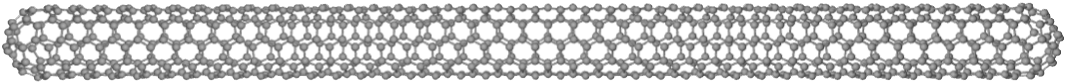
\includegraphics[width=1.0\textwidth]{C840.png}
    \label{pic:toc}
 \end{figure}

\clearpage

%Introduction
\section{Introduction}
{\it Program Fullerene} is a general purpose program that creates a reasonably accurate 3D structure
(cartesian coordinates) for any fullerene isomer through various different methods and algorithms, and subsequently performs a topological/graph 
theoretical analysis. The results can be used for plotting 2D fullerene graphs (Schlegel diagrams) 
and 3D structures, and as a good starting point for further quantum theoretical treatment. The program is 
written in standard FORTRAN and C++ and is easily implemented within a LINUX/UNIX environment.
Although there are several computer programs already available to deal with fullerene graphs 
like {\it CAGE} \cite{Brinkmanx}, {\it FULLGEN} \cite{Brinkman}, {\it BUCKYGEN} \cite{Goedgebeur} or VEGA \cite{Pisanski},
we felt that there is a need to write a general purpose program which does what other programs do and (of course) a lot more. 
In the current version only regular fullerenes are considered (i.e. of genus 0 consisting of pentagons and hexagons only) 
fulfilling Euler's theorem, $n_v - n_e + n_f = 2$, where $n_v$ is the number of vertices (atoms), $n_e$ the number of edges (bonds), and 
$n_f$ the number of faces (5- or 6-rings). The program constructs an accurate 3D structure (cartesian coordinates) of any fullerene isomer 
from the canonical ring spiral pentagon indices (RSPI) through either the 3D Tutte embedding (3D-TE) \cite{Tutte} or the adjacency matrix
eigenvector (AME) method \cite{Atlas}. One can also construct the $n$-th leapfrog $GC_{1,1}^n[C_{n_v}]$ fullerene or a halma fullerene 
$GC_{k,0}[C_{n_v}]$ as a special case of a Goldberg-Coxeter transformation $GC_{k,l}$. Starting from a given fullerene structure one can 
perform vertex insertions (such as Endo-Kroto \cite{Endo92} or Yoshida-Fowler \cite{Yoshida97}), W-S \cite{WS}
or Stone-Wales transformations \cite{Stone86}. 
Vertex insertions allow for the construction of non-spiral fullerenes such as \C{380} or \C{384}. 
Geometry optimization using a Fletcher-Reeves-Polak-Ribiere
minimization with analytical gradients for the Wu force-field \cite{Wu87} is implemented in the current version, providing 
a good initial guess for 3D cartesian coordinates. 2D fullerene graphs (Schlegel diagrams)
can be produced using a variety of different algorithms \cite{Plestenjak}. The program determines the volume and surface area 
of a fullerene (irregular or not) through tesselation in trigonal pyramids or from the convex hull, and gives measures for
spherical distortion and convexity. It determines the minimum covering sphere, the minimum distance sphere
and the maximum inner sphere. The program further calculates the number of Hamiltonian cycles
and produces ring spiral indices. Finally, Cioslowski's scheme for the calculation of the heat of formation for IPR
(independent pentagon rule) fullerenes is implemented \cite{Cioslowski2000}, as well as Babi{\'c}'s scheme for calculating the 
total resonance energy of a general fullerene \cite{Babic1995,Babic1997}, and Martin's scheme for the heat of formation \cite{Alcami}.

This program works for any (distorted or not) regular fullerene. The spiral algorithm of Fowler and Manolopoulus used here \cite{Atlas}
is not restricted to a pentagon start or to canonical indices. For a general list of fullerenes see ``The House of Graphs'' \cite{HouseofGraphs}. 
The program produces an external file with default name {\bf Fullerene-3D.xyz} to be used for standard molecular plotting programs
like CYLview \cite{CYLview}, Avogadro \cite{Avogadro}, Jmol \cite{JMol}, Pymol \cite{Pymol} or VMD \cite{vmd}.  For using these programs 
it is important that the fullerene has a reasonable structure, obtained for example by a force-field 
optimization, otherwise bonds cannot be correctly identified. It may therefore not be advisable to use structures that come out directly from
the AME or 3D-TE algorithm. We recommend CYLview, it is more robust and works for large fullerenes up to about 1000 atoms. 
For larger fullerenes Pymol is recommended. The program produces fullerene 2D graphs in latex format, but can
be used by any other program which is capable of producing 2D graphs, for example QMGA \cite{Gabriel2008}. 
For this an external file is written out called {\bf Fullerene-2D.dat} containing all the information required for plotting a 2D graph.

Version 4.0 (released July 2012) now incorporates C++ routines embedded into the original FORTRAN program using 
much improved algorithms compared to the older version. The reason for using two different program languages is
that PS is good in old-fashioned Fortran and JA is good in C++.  Furthermore, some of the original routines used, were available 
in Fortran only. Some standard routines from Mathematical Recipes were modified for the purpose of matrix diagonalization 
and geometry optimization. This program is under permanent construction and has been tested extensively for bugs.
Nevertheless, if you have any problem or find any bug please report it to one of us.

There are many things on our to-do list. We try hard to release more functionality to this program soon.
Not implemented yet is: 1) The minimum covering ellipsoid useful for  rugby-ball shaped fullerenes (yes this is New Zealand
and crazy about rugby), and close packing of ellipsoids; 2) The general Goldberg-Coxeter (GC$_{k,l}(n)$) construction for fullerenes;
3) Geometry optimization using improved force fields; 4) Frequency calculations from the force-field 
optimized geometry; 5) Construction of non-ring-spiral isomers using a generalized ring spiral algorithm; 6) Symmetry labels for 
H\"uckel orbital energies; 7) Extension to non-classical fullerenes of genus 0 (heptagons and squares); 8) Extension to non-regular fullerenes 
of genus 1 (hmmm, donuts!); 9) To symmetrize optimized coordinates to point group symmetry; 
10) A restart option for subroutine Hamilton; 11) Use of ``House of Graphs'' 
fullerene database; 12) Plotting program (other than latex) for producing Schlegel diagrams and corresponding duals
with a good graphical interface similar to the {\it CAGE} program \cite{Brinkmanx}.

We are also open to any other suggestions and welcome additions to this program suite.


\clearpage
%Installation and running the program
\section{Installation and running the program}
All fortran files are located in the directory ``source'' and all C++ files are in ``libgraph''.

The program is LINUX/UNIX based and is tested to compile with the gnu compiler collection (more specifically gfortran and g++).
You need to use the {\bf Makefile} included in the {\bf fullerene.zip} file provided and type\\\\
\verb|make|

It currently compiles in a 64 bit version, but you can change it in the Makefile to 32 bits if required.
The executable ``fullerene'' runs on a LINUX/UNIX as\\\\
\verb|./fullerene < filename.inp > filename.out|

A number of test input files can be found in the directory ``input''. If you type\\\\
\verb|make tests|

it will run all the input jobs and stores them into the output directory as *.out. If you type\\\\
\verb|make clean|

all the object files are deleted. Additionally, the linked binaries are deleted if you type\\\\
\verb|make distclean|

If you use the fullerene database (which is recommended for time savings), the file needs to be in the directory
where the source and libgraph directories are located.

To use the latex program for the 2D fullerene graphs you need to use the files standalone.cfg and standalone.cls.

%Program Structure
\section{Program Structure}
The main program ({\bf main.f}) calls a number of subroutines for certain tasks and in a certain sequence.
Subroutine {\bf DataIn} manages all the input and determines these main tasks to be carried out.
The input is in {\it Namelist format} if not otherwise stated. 
Important steps in the program are given in the flow diagram below and are
explained in some detail in this section. More information can be obtained in an up-coming review article \cite{PSJA}.

%Figure 1
\begin{figure}[htbp]
   	\centering
	\includegraphics[width=0.9\textwidth]{tree.pdf} 
    \label{pic:flowdiagram}
    \caption{Flow diagram for main program tasks.}
\end{figure}

The most time-consuming steps in the program are the diagonalization of the adjacency matrix (${\cal O}(n^3)$) 
needed for the AME algorithm and the H\"uckel analysis, the force-field optimization for
very large fullerenes ($>$ 2000 atoms), the determination of the number of Hamiltonian cycles
($>$ 80 atoms) (this is an NP-complete problem), the creation of a list of ring-spiral pentagon
indices for all possible isomers with a given vertex count $n_v$ ($>$ 80 atoms), 
and the Tutte embedding algorithm ($>$ 2000 atoms). We try to improve the performance of these algorithms
in our next version.

%Create a 3D structure for a specific fullerene
\subsection{Create a 3D structure for a specific fullerene}

The easiest way to create a 3D structure is of course to read-in cartesian coordinates for a specific
fullerene (see files {\it c20.inp} to {\it c540.inp}), or to construct them internally for the high
symmetry $I_h-$\C{20} or $I_h-$\C{60} isomers (Subroutine {\bf CoordC20C60}, see input files {\it ico.inp},
{\it icoExp.inp}, {\it icoideal.inp}), or to get the cartesian coordinates from input ring-spiral
pentagon-indices PSPI (Subroutine {\bf CoordBuild}) by using either the Fowler-Manolopoulus AME algorithm \cite{Atlas},
or the more reliable 3D-TE algorithm (used by files {\it pentagon1.inp} to {\it pentagon27.inp}),
or from the Goldberg-Coxeter 2-index transformation (triangulation algorithm, input files {\it coxeter1.inp}
to {\it coxeter6.inp}). The 12 pentagon indices can also be obtained from the {\it fullerene
database} if the canonical fullerene number is used as defined in the book ``Atlas of Fullerenes'' by Fowler and Manolopoulus \cite{Atlas,cvetkovic2002} 
(input file {\it database.inp}).

We recommend reading Fowler and Manolopoulus' book \cite{Atlas,cvetkovic2002} for the use of RSPIs and H\"uckel (adjacency matrix) $P$-type eigenvectors 
to construct 3D fullerene graphs.  For the AME algorithm it is critical to get the right 
H\"uckel eigenvectors for the construction of cartesian coordinates \cite{Atlas}. 
The position of the three~$P$-type eigenvectors can be specified (see file {\it pentagon8.inp} for such an example).
If the AME algorithm fails or you cannot find the required $P$-type eigenvectors, you should use our Tutte embedding algorithm,
which (to our opinion) is less troublesome and may be used as the standard method to construct 3D structures.
3D structures can also be obtained from a Goldberg-Coxeter transformation of \C{20}.

It is important that the end-product is viewed by a molecular visualization program. 
We recommend CYLview by Claude Legault \cite{CYLview}, Avogadro \cite{Avogadro}, JMol \cite{JMol}, Pymol \cite{Pymol} or VMD \cite{vmd}. 
Most of these programs are freely available.  For this purpose a file is written to Fullerene-3D.xyz to be used as an input file 
for these molecular visualization programs.

The program sets the barycenter of the fullerene 
to the origin. Using the obtained cartesian coordinates the program calculates the smallest and largest cage diameters and the
moment of inertia, which already gives a measure for distortion from spherical symmetry (Subroutine {\bf Diameter}). 
It produces the distance matrix~ $d_{ij}$ if the print level is set to high (Subroutine {\bf DistMatrix}), and once the 
molecular point group is obtained, the program determines if the fullerene is chiral or not (Subroutine {\bf Chiral}).
Once the cartesian coordinates $(X_i, Y_i, Z_i)$ for each vertex $i=1,\dots, n_v$ is known, all edges are determined by 
analyzing connectivities between the vertices from either given cartesian coordinates or directly from the adjacency matrix 
if a ring spiral input was chosen (Subroutine {\bf Connect}). In any case, one has the adjacency matrix $A_{ij}$ for all vertices at this stage:
\begin{equation}
  \label{eq:adjacencymatrix}
  A_{ij} =
  \begin{cases}
    1 & \text{if vertices $i$ and $j$ are adjacent}\\
    0 & \text{otherwise}
  \end{cases}
\end{equation}

%List of Isomers
\subsection{List of Isomers}
The program can print all general and IPR isomers for a specific fullerene and perform an analysis as introduced 
in the book by Fowler and Manolopoulus \cite{Atlas}, e.g. pentagon indices and 
pentagon number, hexagon indices and strain parameter, NMR information and number of distinct Hamiltonian cycles if 
required. The number of isomers scales polynomially as $n_v^9$, thus it becomes computationally
too demanding for a full isomer list beyond \C{100}. Moreover, the database provided, can be used to print all isomers up to 
\C{100}, and up to \C{120} for all IPR isomers. Fowler and Manolopoulus use a numbering scheme ($N_\mathrm{isomers}= 1,\dots, n_\mathrm{max}$) 
obtained from the natural sequence of canonical RSPIs to distinguish between the different isomers \cite{Atlas}. From their book \cite{Atlas} the
general isomer number can be taken and the RSPIs for a specific isomer up to \C{100} can be read-in from the database provided. 
The numbering scheme for IPR isomers only ($N_\mathrm{isomers}^\mathrm{IPR}= 1,\dots, n_\mathrm{max}$) can also be used up to \C{120}, see input file {\it database.inp}.

%H\"uckel analysis and topological indicators
\subsection{H\"uckel analysis and topological indicators}
From the adjacency matrix $A_{ij}$ a H\"uckel analysis is performed (Subroutine {\bf Hueckel}). This gives you a good hint if the 
fullerene is open or closed shell \cite{Atlas}. For smaller fullerenes or non-IPR fullerenes the H\"uckel analysis may not be very reliable 
as hybridization with the C(2s) orbitals occurs due to non-planarity. Hence the $\sigma-\pi$ separation breaks down. The orbital energies are defined as
\begin{equation}
  \label{Hueckel}
  \epsilon_i=\alpha+x_i\beta
\end{equation}
and we adopt $\alpha = -0.21$ au  and  $\beta = -0.111$ au obtained
from the experimental ionization potential (7.58 eV) and excitation energy (3.02 eV) of \C{60} (the electron goes 
into the second LUMO of $t_{1g}$ symmetry). This gives also orbital energies for \C{60} in reasonable 
agreement with DFT Kohn-Sham orbital energies. The fullerene structure might also undergo a Jahn-Teller distortion adopting a singlet 
ground state instead of one of a higher multiplicity, as this is the case for \C{20}. Such electronic effects are not
captured in this program, and one needs to perform a proper quantum theoretical calculation. The program gives information
on the HOMO-LUMO gap and calculates the topological resonance energy from Babi\'c's matching polynomial calculations \cite{Babic1995,Babic1997}.
There are several other topological indicators of which the Estrada index and mean topological distance, the Wiener index and the hyper-Wiener
index are printed. For details consult a book on graph theory.

%The Goldberg-Coxeter transformation
\subsection{The Goldberg-Coxeter transformation}

In a next step a Goldberg-Coxeter transformation $GC_{k,l}(n)$ for a fullerene \C{n} can be performed if required from the input
(Subroutine {\bf GoldbergCoxeter}). This leads to a fullerene C$_{k^2+kl+l^2}$. The current implementation allows only for
{\it leapfrog transformations} ($k=l=1$) and for {\it halma transformations} ($k \neq 0$ and $l=0$). However, the program allows 
for multiple leapfrog transformations for the construction of very large fullerenes. A general $GC_{k,l}(n)$  for all values of $k$ and $l$ 
is currently in preparation. 

The general Goldberg-Coxeter construction $GC_{k,l}[G_{0}]$ used here works in the following way: ($i$) Consider
a cubic planar graph $G_{0}$ and take its dual (faces become vertices and
vertices become faces), $D_{t}(G_{0})$. This transforms the graph $G_{0}$
with $n_v$ vertices into a triangulation, i.e. a geodesic sphere with $n_v$ triangles; (\textit{ii})
Each triangle $T_{k}$ ($k=1, \dots, n_{v}$) of the geodesic sphere is
subdivided into another set of faces $t_i$ using the Coxeter indices ($k,l$).
If the obtained new smaller faces $t_i$ are not
triangles themselves within one $T_k$, when neighboring $T_k$s are glued
together with other non-triangle faces, new triangles are formed and we end up with a new triangulation,
i.e. a larger geodesic sphere $GC_{k,l}D_{t}(G_{0})$;
(\textit{iii}) Finally we take the dual which yields a new fullerene,
\begin{equation}
 	G_1 = GC_{k,l}[G_0] = D_t GC_{k,l} D_t(G_0)
	\label{eq:GC}
\end{equation}

If the initial graph $G_0$ has $n_v$ vertices, the number of vertices of $GC_{k,l}[G_0]$ is
\begin{equation}
	n_v^{GC} = t(k,l)n_v = (k^2 + kl + l^2)n_v
	\label{eq:GCvertexcount} 
\end{equation}
$t(k,l)$ is called the {\em triangulation number}. We work with the dual triangulation instead of a hexagonal mesh as it is easier to implement.

%Hamiltonian cycles
\subsection{Hamiltonian cycles}
Subroutine {\bf Hamilton} uses the back-track algorithm of Babi\'c \cite{Babic1995a} to obtain all 
Hamiltonian cycles and subsequently (if required) the IUPAC name of the fullerene. Hamiltonian cycles go through all vertices exactly once returning 
to the starting point. The number of distinct Hamiltonian cycles has carefully been checked 
against a second algorithm for various fullerenes, and left-right cycles and cyclic vertex permutations counted as the 
same. Although finding all Hamiltonian cycles is an NP-complete problem, the algorithm works fine up to about \C{100}. 
After that it becomes computationally very demanding. Therefore, for the larger fullerenes the program prints upper and lower limits instead. The existence of Hamiltonian cycles for fullerenes is only conjectured at this stage, and only for layered fullerenes 
(e.g. fullerene with onion-shaped 2D graphs such as nanotubes) existence has been proven. Our recent calculations verified that
Hamiltonian cycles exist for all fullerene isomers up to \C{100} and for all IPR isomers up to \C{120} \cite{PSAJDB}.

%Force-field optimization
\subsection{Force-field optimization}
The geometry can be optimized by force fields using a Fletcher-Reeves-Polak-Ribiere geometry optimization \cite{NumRec}
with analytical gradients (Subroutine {\bf OptFF} \cite{NumericalRecipes}). In the currently version the Wu
force field is implemented, which considers bond lengths and angles only in an harmonic oscillator approximation \cite{Wu87}: 
\begin{equation}
  \label{eq:Ewu}
  E_{\mathrm{Wu}} = \frac{k_p}{2} \sum_{i_p}^{\mathrm{edges}} \left(R_{i_p} - R_p\right)^2 
        + \frac{k_h}{2} \sum_{i_h}^{\mathrm{edges}} \left(R_{i_h} - R_h\right)^2 
        + \frac{f_p}{2} \sum_{j_p}^{\mathrm{ring}} \left(\theta_{j_p} - \theta_p\right)^2 
        + \frac{f_h}{2} \sum_{j_h}^{\mathrm{ring}} \left(\theta_{j_h} - \theta_h\right)^2 
\end{equation}
Only bonded pairs of vertices are taken into account. $k_{p}$ and $k_{h}$ are
the force constant for the two different C--C bonds (set to $\approx 300 \text{\,kcal\,\AA}^{-2}$), $R_p$ and $R_h$ the corresponding pentagon and
hexagon bond distances ($\approx$ 1.4 \AA), and $\theta _p $ and $\theta _h$ are the corresponding bond angles (108$^\circ$ and 120$^\circ$
respectively).

The force-field optimization is very fast even for fullerenes such as \C{840}. 
The Wu force-field optimization may lead to distortions of the fullerene to a structure of lower symmetry compared to the original point-group. 
Moreover, as no
dihedral angles are fixed, the molecule might distort away from convexity. In such cases an additional Coulomb repulsive potential can
be added (see input instructions) in a preoptimization step,
\begin{equation}
  \label{eq:Ewu}
  E = E_{\mathrm{Wu}} + E_{\mathrm{Coulomb}} = E_{\mathrm{Wu}} + \sum_{i=1}^{\mathrm{vertices}} \frac{f_{\mathrm{Coulomb}}}{|r_i - r_0|}
\end{equation}
with $r_i - r_0$ being the distance between vertex $i$ and the barycenter.
Note that the construction of the fullerene by using the AME or Tutte algorithm may
lead to a more spherical arrangement prior to a force-field optimization with rather large bond distances, 
e.g. barrels instead of nanotubes. A more sophisticated force field using dihedral angles is currently being developed.

%Ring connectivities, patterns, vertex insertions and spiral detection
\subsection{Ring connectivities, patterns, vertex insertions and spiral detection}
Subroutine {\bf Ring} identifies all pentagons and hexagons (faces) and checks if Euler's theorem is fulfilled.
Subroutine {\bf RingC} then determines the center for each pentagon and hexagon later used for the trigonal pyramidal tessellation to obtain
the fullerene volume and surface. This routine also analyzes all 2- and 3-ring fusions and many other useful patterns needed for example
in Stone-Wales transformations or vertex insertions. It further determines the Rhagavachari-Fowler-Manolopoulos neighboring pentagon 
and hexagon indices as described in detail in Fowler and Manolopoulos' book \cite{Atlas}.
From the hexagon indices one derives if the fullerene is IPR or not. If it is IPR, Cioslowski's scheme is used to calculate the 
heat of formation \cite{Cioslowski2000}. For all fullerenes, Martin's scheme is used to calculate the heat of formation \cite{Alcami}.

Information from subroutine {\bf RingC} can be used to perform Stone-Wales transformations \cite{Stone86}
(subroutine {\bf StoneWalesTrans}), Endo-Kroto 2-vertex insertions \cite{Endo92} (subroutine {\bf EndoKrotoTrans}),
Yoshida-Fowler 4-vertex ($D_{3h}$ 6555) (subroutine {\bf YoshidaFowler4}) and 6-vertex ($D_{3h}$ 666555)
insertions (subroutine {\bf YoshidaFowler6}) \cite{Yoshida97}, or the a WS 6-vertex (6-55-55) insertion 
we developed, see input files {\it c50EK.inp, c60SW.inp, c80YF.inp}. 
Non-spiral fullerenes such as  \C{380} or  \C{384} can be constructed with these vertex insertion methods, see input files {\it c380.inp} 
and {\it c384.inp}. The two structures obtained from a force-field optimization are shown in Figure \ref{pic:C380andC384} using program PYMOL \cite{Pymol}.

%Figure 2
 \begin{figure}[htbp]
   	\centering
  	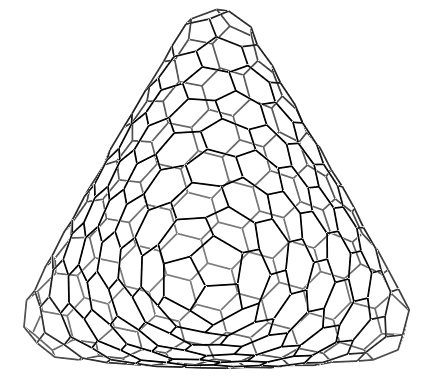
\includegraphics[width=0.3\textwidth]{C380.png}
	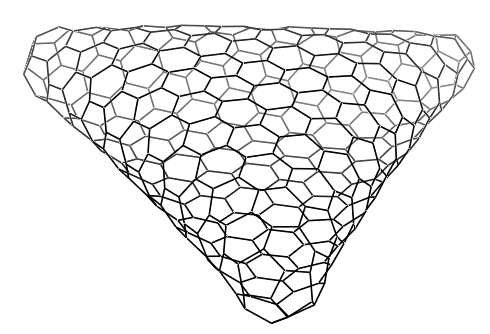
\includegraphics[width=0.4\textwidth]{C384.png}
    \caption{Optimized force-field structures of \C{380} (left) and \C{384} (right).}
	\label{pic:C380andC384}
 \end{figure}

Subroutine {\bf SpiralSearch} uses the ring-spiral algorithm of Fowler and Manolopoulus \cite{Atlas}
for the search of a ring spiral if, for the input, cartesian coordinates were chosen, or if the
initial fullerene structure was modified. It produces the canonical ring spiral pentagon indices
if the fullerene is spirable and fails if it is non-spirable (as for the two examples shown in 
Figure \ref{pic:C380andC384}.  A more general ring-spiral algorithm is currently in preparation.

%Volume and surface area, minimum covering sphere
\subsection{Volume and surface area, minimum covering sphere, \\ minimum distance sphere and maximum inner sphere}
The volume and surface area of the fullerene are calculated in Subroutine {\bf Volume}. This is done by\\
1) The convex hull.\\
2) The normal vector algorithm resulting in the exact volume of the polyhedron (identical to convex hull if polyhedron is convex).\\
3) The tesselation into trigonal pyramids from the barycenter by summing over all tetrahedrons spanned
by the three vectors (identical to algorithm 1 and 2 if the polyhedron is convex).  A sum over all
tetrahedrons spanned by the three vectors CM-CR (center(mass)-center(ring): barycenter of fullerene to the ring center),
CM-CA1 (barycenter of fullerene to atom~1 in ring), and CM-CA2 (barycenter of fullerene  to atom~2 in ring) is calculated.
There are 5 such tetrahedrons in a pentagon and 6 in a hexagon.  The barycenter CM has been set to the origin in a previous step.

In a similar way the surface area is obtained by summing over all triangles from the ring center to
neighbouring vertices in the ring. $I_h$-\C{20} and $I_h$-\C{60} coordinates can be constructed easily
using basic geometry. For these, the volume and surface areas are known analytically.

The {\it isoperimetric quotient} (IPQ) is defined as
\begin{equation}
 q_{\textrm{IPQ}} =36\pi \frac{V^{2} }{S^{3}}\quad\text{with}\quad q_{\textrm{IPQ}}\in [0,1]
 \label{IPQ}
 \end{equation}
which for an ideal sphere is trivially $q_{\textrm{IPQ}}=1$, and for zero volume $q_{\textrm{IPQ}}=0$. For \C{20} 
and \C{60} with equal bond lengths we get
\begin{equation}
\label{IPQC20}
q_{\textrm{IPQ}} (\C{20}) =0.75470 
\end{equation} 
\begin{equation}
\label{IPQC60}
q_{\textrm{IPQ}} (\C{60}) =0.90317 
\end{equation} 

 We can now define the deviation from a sphere (in \%) by
\begin{equation} 
D_{\textrm{IPQ}} =100\left(1-q_{\textrm{IPQ}} \right) 
\end{equation}

The program also calculates the {\it sphericity parameter} of Diaz-Tendero \cite{Diaz},
\begin{equation}
\label{Diaz}
q_{\textrm{SP}} = \sqrt{(A-B)^2+(A-C)^2+(B-C)^2}/A 
\end{equation}
where $A \ge B \ge C$ are the rotational constants. Note that we deviate from the original definition by dividing 
the square-root by the rotational constant $A$. Further, the {\it asymmetry parameter} of Fowler is printed,
\begin{equation}
\label{Diaz}
q_{\textrm{AP}} = \sum_{i=1}^{n_v}  \frac{(r_i-r_0)^2}{r_0^2}
\end{equation}
where $r_i$ is the radial distance of atom $i$ from the barycenter and $r_0$ is the average distance \cite{Fowler2000}.

Three routines follow to calculate the {\it minimum covering sphere} (MCS) of a fullerene (Subroutine
{\bf MinCovSphere2}) using algorithm 2 of Yildirim \cite{Yildirim08}, {\it minimum distance
sphere} (MDS) (Subroutine {\bf MinDistSphere}), and the {\it maximum inner sphere} (MIS) (Subroutine {\bf MaxInSphere}).
The MCS is defined as follows:
Let $S = \vec{p}_i$ be the set of $n$ points ($i=1,\ldots ,n$) in $m$-dimensional Euclidean space, 
$R^m$. The MCS of this set, MCS($S$), is a sphere of smallest radius $R_{MCS}$ that encloses the set of points $S$,
and can be expressed as follows,
\begin{equation}
	\label{eq:MCS}
	\min\limits_{\vec{c}_{\mathrm{MCS}} } \max\limits_i \left\| \vec{p}_i -\vec{c}_{\mathrm{MCS}} \right\|  
\end{equation} 
where $\|\cdot\| $ denotes the Eucledian norm and $\vec{c}_{\mathrm{MCS}}$ is the center of the MCS. The MCS
is uniquely defined and can be expressed as a convex combination of at most 
($m+1$) points, hence our algorithm stops when 4~points are left over in the iteration process of the algorithm.
The spherical central cover SCC is not the minimum covering sphere MCS
(except for example if all distances from the barycenter CM are the same as in the
ideal capped icosahedron). The spherical central cover is taken from the
CM point with radius $R_{\mathrm{max}}$ (longest distance to one vertex).  We changed the first
condition in this Yildirim's algorithm by choosing the furthest point from CM.
In the final statistics there should be 0 points outside the sphere and at least 1 point on the sphere.
We can now introduce the definition for the MCS distortion parameter $D_{MCS}$ (in \% of $r_{\mathrm{min}}$),
\begin{equation} \label{eq:DMCS}
D_{\mathrm{MCS}} =\frac{100}{n_vr_\mathrm{min}} \sum_{i=1}^{n_v} \left(R_{\mathrm{MCS}} - \|\vec{p}_i - \vec{c}_{\mathrm{MCS}}\|\right)
\end{equation} 

At the end, the Van der Waals radius of carbon (1.415\,\AA) is added to the radius of the MCS
(Input coordinates for this need to be in \AA{} otherwise you are required to change the program),
and the volume of an ideal fcc solid is calculated. The Van der Waals radius is chosen such that
for \C{60} the solid-state results of Heiney et al. \cite{Heiney91} are reproduced.
In the case of nonplanar pentagons or hexagons there is no unique definition for the volume of a fullerene,
except for the convex hull. There is no reason, however, why any other definition should be preferred
over the exact volume algorithm employed in this program.

The MCS is biased for the case that few atoms stick out on the surface of a fullerene,
and the minimum distance sphere (MDS) may be more appropriate for a measure from spherical distortion,
\begin{equation} 
\min\limits_{c_\mathrm{MDS} \in CH(S)} \frac{1}{n_v} \sum _{i} \left|R_\mathrm{MDS} -\left\| \vec{p}_{i}-\vec{c}_{MDS} \right\| \right|  
\end{equation}

with the MDS radius
\begin{equation} 
	R_{\mathrm{MDS}} =\frac{1}{n_v} \sum _{i}\left\| \vec{p}_{i} -\vec{c}_{\mathrm{MDS}} \right\|   
	\label{eq:RMDS}
\end{equation} 

The restriction of $\vec{c}_{\mathrm{MDS}}$ to be inside the convex hull is necessary as $\vec{c}_{\mathrm{MDS}}$ may move
out of the fullerene structure in the optimization procedure.  In general we have $\vec{c}_{\mathrm{MDS}}\ne\vec{c}_{\mathrm{MCP}}$
except for the case that all points lie on the MCS. The MDS may however not be uniquely defined, as there could be many 
(even degenerate) local minima, but for most case (i.e. ``spherical'' fullerenes) it works just fine.  
This gives a better definition for the distortion
parameter compared to $D_{\mathrm{MCS}}$, as it is not biased to a few points lying outside or inside the fullerene surface.
Hence, analogous to the MCS we define a measure for distortion from spherical symmetry through the MDS,
\begin{equation}
  \label{eq:DMDS}
  D_{\mathrm{MDS}} = \frac{100}{n_v r_{\mathrm{min}}} \sum_{i=1}^N \left|R_{\mathrm{MDS}} - \|\vec{p}_i - \vec{c}_{\mathrm{MDS}}\| \right|
\end{equation}

The maximum inner sphere (MIS) is important to estimate if there is enough space inside the fullerene cage for endohedral atoms or molecules. It is
defined as
\begin{equation}
	\max\limits_{c_{\mathrm{MES}} \in \mathrm{CH}(S)} \min\limits_{i} \left\| \vec{p}_{i} -\vec{c}_{\mathrm{MES}} \right\|  
	\label{MES} 
\end{equation}

For ideal \C{60} ($I_h$ symmetry) MCS, MDS and MES are all identical. 
For the MIS the radius and volume is printed  with the Van der Waals radius of carbon taken off $R_{\mathrm{MIS}}$. 

%2D fullerene graphs and Schlegel diagrams
\subsection{2D fullerene graphs and Schlegel diagrams}
Fullerenes can be nicely visualized by 2D fullerene graphs. They should be distance-transitive, distance-regular and 
symmetric. There are a number of different algorithms available trying to achieve this, and in subroutine {\bf Graph2D} $(X_i,Y_i) (i=1,\dots, n_v)$ 
coordinates for a 2D fullerene graph are created. Here we briefly describe the algorithms we recommend to use,
others are of perhaps of more historical interest. Note that for non-spherical fullerenes (like the famous non-spirable \C{380} (Figure  \ref{pic:C380andC384})
tetrahedron) it becomes very difficult to create a good Schlegel projection, and in such cases the projection of vertices to the minimum
covering sphere is recommended before these algorithms are used (see input). The subroutine produces latex file with the fullerene graph included.

1) The perspective Schlegel projection (SP): Here the points are rotated such to put a selected vertex, edge or ring center 
on top of the $z$-axis just below the projection point (otherwise the point $(0,0,z_{\mathrm{max}})$ is chosen with $z_{\mathrm{max}}$
being the point with maximum $z$-value from the original input coordinates). Points are then sorted in descending order according to their z-values.
The circumference for atoms and rings down the z-axis are determined. The Schlegel projection is created giving as output the projected $(X_i,Y_i)$
coordinates, i.e. points are projected down a plane from a set projection point. 
The connections between the points are already written out earlier in the output such that the fullerene graph can be drawn.
There are two choices for the projection, depending if you choose the outer ring or the center part of the fullerene graph as a starting point:
    
2) The cone projection (CSP), i.e. points are projected out to an enveloping cone and then down to a plane below the fullerene. 
The last ring center should be at the bottom of the fullerene and if detected, will not be projected 
out, or if not will have a large scale factor (this center may be ignored in the drawing). Also, the 
last points on the outer ring in the fullerene graph are scaled in distance by 1.2 in order to make the outer rings 
more visible. This also moves the outer centers within the ring.
       
At the end a rough plot of the fullerene graph is produced. This is suitable for fullerenes up to about \C{100}, beyond that
it becomes too crowded and the latex file produced contains a better graph. Nevertheless, it serves for a first rough picture. 
Furthermore, for large fullerenes it becomes critical to correctly set the projection point or point of the cone.
If, for example the projection point is too far away from the fullerene, edges may cross.

3) Tutte 2D embedding with linear scaling (2D-TE-LS). Here the Tutte algorithm is used \cite{Tutte}
but the resulting overcrowding of small polygons near the center of the graph is remedied
by a linear scaling procedure
\begin{equation}
	\label{GrindEQ__16_} 
	\lambda_i = 1+\frac{f(r_\mathrm{min} - r_i)}{r_\mathrm{min}}
\end{equation}
applying a linear scaling factor $\lambda_i$ to all vertices $v_i$ ($i=5(6),\dots , n_v$), where $f$
is a parameter to be determined, $r_{\mathrm{min}}$ is the smallest distance to the vertices of the peripheral
taken from the barycenter $P$ of the innermost ring (or alternatively the barycenter of the 2D convex hull), 
and $r_i$ is the distance from that point $P$ to the vertex $v_i$.

4) Pisanski-Plestenjak-Graovac embedding algorithm (PPGA) \cite{pisanski95}. This is one of the more successful algorithms developed by 
Pisanski, Plestenjak and Graovac in conjunction with a simulated annealing procedure for better visualization of graphs, 
which is an improvement over usual spring embedders. Here the potential between adjacent vertices is modeled by
\begin{equation} 
\label{eq:Eppg} 
E_{\mathrm{PPG}} =\sum_{i<j}^{\mathrm{ord}(G)} A_{ij}  r_{ij}^{2} \exp \left(\alpha \frac{2d_{\mathrm{max}} -d_{iP} -d_{jP} }{d_{\mathrm{max}} } \right) 
\end{equation} 
where $A_{ij}$ is the adjacency matrix, $r_{ij}$ the distance between vertex $i$ and $j$, and $\alpha$ a
parameter to be determined. The distances in eq.\eqref{eq:Eppg} are defined through the topological
distance matrix $D$,
\begin{equation}
	\label{GrindEQ__20_}
  	d_{\mathrm{max}} = \max_{j,j_P}\left\{ D_{ij_P} \right\}\quad\text{and}\quad d_{ip} = \min_{j_P}\left\{ D_{ij_P} \right\}
\end{equation}
where  $j_P$ is the vertex number belonging to the (5 or 6) peripheral vertices.  Instead of a
simulated annealing algorithm we start with a Tutte 2D graph and perform a minimization procedure for $E_{\mathrm{PPG}}$.

For other 2D graph embedding methods implemented see the following input section.
       

%Input description
\section{Input description}

Input and output files are in the directories {\it input}  and   {\it output}  respectively. {\it Program Fullerene} has been tested 
for many fullerenes found in the following input files:
\C{20} (c20.inp), \C{24} (c24.inp), \C{26} (c26.inp), \C{28} (c28.inp), \C{30} (c30.inp),
\C{36} (c36.inp), \C{50} (c50.inp), \C{60} (c60.inp), \C{70} (c70.inp), \C{72} (c72.inp),
\C{74} (c74.inp), \C{78} (c78.inp), \C{80} (c80.inp), \C{92} (c92.inp), \C{100} (c100.inp),
\C{180} (c180.inp), \C{320} (c320.inp), and \C{540} (c540.inp), and the non-spirable fullerenes \C{380} (c380.inp) 
and \C{384} (c384.inp). Input files pentagon1.inp to pentagon25.inp are for
RSPI inputs. Many more examples can be found. The cartesian coordinates used in the input files are mostly singlet electronic state 
B3LYP aug-cc-pVDZ optimized up to \C{60}, cc-pVDZ up to \C{180}, and 6-31G for the rest. 
For some of the fullerenes listed, the singlet state chosen may not be the electronic ground state.
Many definitions depend on the use of {\AA}ngstr{\o}ms for distances, so please use this unit throughout. 
A typical input is in {\it Namelist format}, or if additional data are required in {\it free format}, and reads like this:\\\\
C80  Using FM algorithm to produce coordinates, input file: pentagon12.inp \\
\&Coord NA=80, ICart=2, IV2=4, IV3=5 / \\
\&FFChoice Iopt=1 / \\
\&FFParameters / \\
\&Hamilton IHam=1 / \\
\&Isomers IPR=1 / \\
\&Graph ISchlegel=2, ISO1=2, ISO2=4, ISO3=5 / \\
1 2 3 4 5 6 37 38 39 40 41 42 \\\\
The first line is a text line, the second \&Coord line in {\it namelist format} tells the program how the coordinates are created (and many more), the
next two lines \&FFChoice and \&FFParameters are specifications for the force field to be used (none in this case), line 4 (\&Hamilton) concerns the
Hamiltonian cycles, line 5 (\&Isomers) is an isomer list is created, and line 6 (\&Graph) for the 2D fullerene graph (Schlegel diagram). The last
line in the input is for the 12 ring-spiral pentagon indices (RSPI).

In the following, the input in the required sequence is described in detail (either Namelist or in Free Format):\\\\

1) {\bf Text line} of max. 132 characters (in 132A1 format) (you can put as many text cards into the input as you want).\\\\

2) {\bf \&Coord line}: Input to create cartesian coordinates and main flags for the program (e.g. \&Coord ICart=20, R6=1.42 /).\\
{\it List of options:}\\ 
{\bf NA, ICart, IV1, IV2, IV3, ixyz, filename, isonum, ichk, leap, GCtrans, kGC, lGC, ISW, KE, IYF, ISW, ihueckel, ipsphere, loop, mirror, IP, IPRC, TolR, R5, R6}\\
{\bf NA} = Number of atoms (vertices) $N_A$ (Default: 60)\\
{\bf ICart} = Flag for the construction of the 3D structure (cartesian coordinates) (Default: 0). For more details see below.\\
{\bf IV1} = Number for H\"uckel P-type eigenvector for AME algorithm (Default: 2)\\
{\bf IV2} = Number for H\"uckel P-type eigenvector for AME algorithm (Default: 3)\\
{\bf IV3} = Number for H\"uckel P-type eigenvector for AME algorithm (Default: 4)\\
{\bf filename} = 'name'. Filename for all external files created or used by the program.\\
{\bf ixyz} = Flag for producing .xyz input file for CYLview, Avogadro or other plotting programs in standard xyz format (Default: 0). 
Default name for the external file is {\it Fullerene-3D.xyz}. Otherwise {\bf filename}='filename' needs to be specified (max 20 characters).\\
{\bf isonum} = Isomer number according to the scheme introduced in Fowler and Manolopoulus' book \cite{Atlas} (Default: 0).\\ 
If {\bf ICart} = 2, 3 or 4 and {\bf isonum} not zero, then pentagon indices are taken from the
isomer list contained in a database (see below).\\
There are two databases, one for the general isomers
({\bf IPRC} = 0), and one for the IPR isomers ({\bf IPRC} = 1), the definition is similar to the IPR parameter below (Default: 0).\\
{\bf ichk} = Flag for producing or reading a .xyz file for CYLview, Pymol, Avogadro or other plotting programs (Default: 0).\\
If {\bf ixyz} = 1:  Produce xyz file named {\bf filename-3D.xyz} for further input.\\
If {\bf ixyz} = 2:  Read xyz from file specified in {\bf filename}. {\bf ICart} = 0 needs to be specified for this. Another xyz file is also produced 
and named   {\it filename-3Dnew.xyz}.\\
If {\bf ixyz} = 3  Read xyz from file specified in {\bf filename}. {\bf ICart} = 0  needs to be specified.\\
{\bf filename}: A name of up to 13 characters must be chosen, the file is then named filename-3D.xyz (Default: Fullerene-3D.xyz).
If {\bf ICart} = 2, 3 or 4 and {\bf isonum} not zero, than pentagon indices are taken from the isomer list contained in a database (see below). 
There are two databases, one for the general isomers ({\bf IPRC} = 2) and one for the IPR isomers ({\bf IPRC} = 1), the
definition is similar to the {\bf IPR} parameter below (Default: 2).\\
If {\bf leap} = $n_{leap}$ the initial fullerene C$_{N_A}$ is subjected to an $n-th$ leapfrog transformation. 
This converts the number of atoms $N_A$ to $N^{'}_A = 3^{n_{leap}}N_A$. (Default: 0)\\
If {\bf GCtrans} = 1 the initial fullerene structure is subjected to a Goldberg-Coxeter transformation $GC_{k,l}$[C$_{N_A}$] (Default: 0).
At the moment only $l=0$ is implemented, also the leapfrog transformation $k=1$ and $l=1$ is available in this input.
In this case {\bf kGC} in the namelist input has to be specified. \\
If {\bf IWS} = 1 the initial fullerene structure is subjected to a Stone-Wales transformation (Default: 0). In this case an
input is required (after all the other input, last card) with pairs of
pentagon ring numbers. Numbers are between 1 and 12. These can be obtained
from a previous output in the section where ring connections are analyzed
and Stone-Wales patterns are printed. In the output for Stone-Wales
numbers the first and last ring numbers are the ones required as these
are the pentagons. Alternatively you can set the second number to zero,
the first number now determines that the Nth Stone-Wales pattern found in the list is taken.
For example, an input\\     
2 3 5 0\\
means pentagon 2 and 3 is taken and the 5th in the printed list of Stone-Wales patterns (see output).\\
If {\bf KE} = 1 the initial fullerene structure is subjected to a Endo-Kroto 2-vertex insertion (Default: 0).
In this case an input is required (after all the other input, last card) with pairs of
pentagon ring numbers. Numbers are between 1 and 12. These can be obtained
from a previous output in the section where ring connections are analyzed
and Endo-Kroto patterns are printed. Input is equivalent to the Stone-Wales transformation described above.\\
If {\bf IYF} = 1 or 2 then a Yoshida-Fowler 4-vertex insertion \cite{Yoshida97} is performed (Default: 0). 
In this case an input is required  with either hexagon numbers (IYF=1) or the position in
the list of Yoshida-Fowler patterns given in the output (IYF=2).\\
If {\bf IYF} = 3 or 4 then a Yoshida-Fowler 6-vertex insertion \cite{Yoshida97} is performed (Default: 0). 
In this case an input is required with the three hexagon numbers (IYF=3) or the position in
the list of Yoshida-Fowler patterns given in the output (IYF=4).\\
If {\bf ISW} = 1 the initial fullerene structure is subjected to a 9-vertex insertion (Default: 0).
Similar to Yoshida-Fowler, an input is required (see {\it c384.inp} for details).\\
If {\bf ihueckel} = 1 diagonalization of H\"uckel matrix is avoided which is of order $O(n^3)$ (recommended for large matrices
over size 5000) (Default: 0).\\
If {\bf ipsphere} = 1 all vertices are projected onto the minimum covering sphere useful for drawing 2D fullerene graphs (Default: 0).\\
If {\bf ipsphere} = 2 In addition an xyz file is written out named filename-3DMCS.xyz (Default: Fullerene-3DMCS.xyz).\\
If {\bf loop} = 1: New input required (compound job), i.e. program does not stop at the end but loops back to the beginning (Default: 0). 
This is important if one takes an initial structure and subjects it to further transformations, for example in subsequent Stone-Wales or
Goldberg-Coxeter transformations. You might use this option to read from a xyz file created in the previous run.\\
If {\bf loop} = 2: Same as above but if ICart specified correctly, it takes pentagon indices from a previous run.\\
If {\bf mirror} = 1 invert all coordinates (take the mirror image). This may be important for chiral fullerenes (Default: 0).\\
If {\bf IP} = 1 Print option for larger output to be produced, i.e. the full distance matrix, all Hamiltonian cycles 
and all 3-ring connections (Default: 0).\\
{\bf IPRC}: see entry for {\bf isonum}.\\
{\bf TolR} = Tolerance in \% (Default: 33). Only change this parameter if the program cannot produce correctly the adjacency matrix. 
This is only necessary for the cartesian coordinate input ({\bf ICart}=1) and only fails if bond distances are unusually large or small. 
Connectivities are found for atoms with distances between R6   and   R6*(1+TolR/100). If TolR=0.0 the default value of 33\% is used. 
If this parameter is set at a value too large, unwanted connectivities
are produced resulting in smaller polygons. This parameter should reflect the maximum deviation in distance from the smallest distance found.\\
{\bf R5} = pentagon bond distance, i.e. the bond length in the pentagons (Default: 1.455).\\
{\bf R6} = hexagon  bond distance, i.e. the bond length of the bonds connecting hexagons (Default: 1.391).  
If {\bf R5} = {\bf R6} is chosen then the ideal capped icosahedron for \C{60} is obtained if NA=60 is chosen.\\\\
More details for the {\bf ICart}-flag:\\
If {\bf ICart} = 0 No coordinate input required, coordinates are constructed for the IPR isomer of \C{60} (or \C{20} if NA=20 is chosen).
You may like to specify R5 and R6 in the input, otherwise the default values are taken.\\
If {\bf ICart} = 1 Cartesian Coordinates expected as input. In this case NA extra lines are required with\\\\
$N_{Z_i}, X_i, Y_i, Z_i$  (in free format)\\\\
Here $N_{Z_i}$= Nuclear Charge, and $X_i, Y_i, Z_i$ are the cartesian coordinates for atom $i$ in \AA. NB: $N_{Z_i}$ is not really needed by the program, 
but you can copy easily .xyz files or outputs from other quantum theoretical programs into the input.\\
If {\bf ICart} = 2 or 3 the adjacency matrix is created from a ring-spiral pentagon list. Extra input required (free format):\\\\
$n_{\mathrm{RSPI}}(I), I=1,12$ \\\\
$n_{\mathrm{RSPI}}(I)$ are the 12 Fowler-Manolopoulus ring-spiral pentagon indices which uniquely identify the locations of the 
pentagons if the fullerene is spirable \cite{Atlas}. Use the canonical pentagon ring indices if possible (transformation to the canonical
from should work as well).\\
If {\bf ICart} = 4 or 5 adjacency matrix is created from a Goldberg-Coxeter transform of \C{20}, i.e. $GC_{k,l}$[\C{20}].  At the moment
the program is restricted to $l=0$. In this case the parameter {\bf kGC} in the namelist input has to be used.\\
If {\bf ICart} = 2 or 4 the AME algorithm using $P$-type eigenvectors produced from the adjacency matrix to get cartesian coordinates. 
If the $P$-type eigenvectors are not in sequence
(position 2,3 and 4, see ref.\cite{Atlas} for details), three integer values {\bf IV1, IV2, IV3} can be specified in the \&Coord
namelist input identifying the position of the eigenvectors (see pentagon8.inp for such an example).
In this case a warning occurs which means you should carefully check the eigenvectors used and cartesian coordinates produced.
Otherwise coordinates produced are useless. This is more often the case as you might expect.\\
If {\bf ICart} = 3 or 5 the Tutte embedding (3D-TE) algorithm is chosen for the construction of the 3D fullerene structure from the adjacency matrix. 
This should always work, although the fullerene created might be too spherical compared to the AME algorithm. But this algorithm is easier, 
and (in theory) should never fail. Examples are given in the input files starting with ``pentagon''.\\\\

3) {\bf \&FFParameters and \&FFParameters  lines}: Options for force-field optimization.\\
{\it List of options} for \&FFChoice line: {\bf Iopt, ftol}\\
{\it List of options} for \&FFParameters line: {\bf fCoulomb, WuR5, WuR6, WuA5, WuA6, WufR, WufA, ExtWuR55, ExtWuR56, 
ExtWuR66, ExtWuA5, ExtWuA6, ExtWuDppp, ExtWuDhpp, ExtWuDhhp, ExtWuDhhh, ExtWufR, ExtWufA, ExtWufD}\\
{\bf Iopt} = Flag for force-field optimization (Default: 0)\\
If {\bf Iopt} = 1  then fullerene is optimized using the force field method of Wu et al. \cite{Wu87} within a 
Fletcher-Reeves-Polak-Ribiere algorithm to find the minimum structure. 
There are more sophisticated force fields available \cite{Ceulemans,Hands04},
e.g. {\it Avogadro} has a more sophisticated force-field which you can use, but the Wu force field does the 
job to create good initial cartesian coordinates for further refinement using more sophisticated QM methods. 
A converged energy $E$ much greater than zero (i.e. $E$>0.5) implies that the set distances and angles in the Wu force field cannot be
reached for all atoms and rings.\\
If {\bf Iopt} = 2  Preoptimize with input force field, then optimize with standard Wu force field. This is especially useful for {\bf fcoulomb} 
input (see below).  \\
{\bf ftol}: The convergence tolerance on the energy (Default: $5.0 \times 10^{-8}$)
{\bf WuR5, WuR6, WuA5, WuA6, WufR, WufA} are force-field parameters for Wu force field for
distances R5, R6, and angles A5, A6. The force constants are: distance WufR and
angles WufA (see paper by Wu et al. for details \cite{Wu87}). Defaults: {\bf WuR5} =  1.455, {\bf WuR6} = 1.391, {\bf WuA5} = 1.08d2, 
{\bf WuA6} = 1.2d2, {\bf WufR} = 1.d6, {\bf WufA} = 1.d5
If {\bf fCoulomb} $>$ 0.0 then add an additional repulsive Coulomb force from the barycenter to all atoms (Default:  {\bf fCoulomb} = 0.d0)
This is extremely useful for an initial geometry optimization to keep the fullerene cage convex if for example the Tutte construction leads to not
a good guess of the initial structure. In such cases {\bf fCoulomb} = 100.0 is a good choice.\\\\

4) {\bf \&Hamilton line}: Option for calculating Hamiltonian cycles and IUPAC numbers.\\
\&Hamilton options: {\bf IHam}, {\bf IUPAC}\\
If {\bf IHam} > 0 Then Subroutine HAMILTON is called (Default: 0).\\
If {\bf IHam} = 1 Routine will stop after 1 million Hamiltonian cycles are found.\\
If {\bf IHam} = 1000000000 Program runs forever and prints if IHam is reached (dangerous choice).\\
If {\bf IUPAC} = 1 IUPAC numbers are produced (Default: 0).\\
Only with this option together with {\bf IP} = 1 in the \&Coord input all Hamiltonian cycles are printed. 
{\bf IP} = 0 only gives the best cycle (see Babi\'c \cite{Babic1995a}).
If {\bf IUPAC} = 0 the program goes into a fast subroutine and prints only the total number of Hamiltonian cycles.\\\\

5) {\bf \&Isomers line}: Option for producing list of isomers and properties.\\
\&Isomers options: {\bf IPR}, {\bf IPH}, {\bf IStop}, {\bf IChk} (Default 0 for all options).\\
If {\bf IPR} $>$ 0 then the ring-spiral subroutine of Fowler and Manolopoulus is used \cite{Atlas}.
This sub-program catalogues fullerenes with a given number of vertices using the spiral algorithm and a uniqueness test
based on equivalent spirals. The required input is IPR.\\
If {\bf IPR} = 1 for isolated-pentagon isomers from \C{60} onwards.\\
If {\bf IPR} = 2 for general isomers (this generates a large output and takes some computer time for fullerenes larger than \C{80}).
Also the database has all this information (see below) up to \C{100}.\\
If {\bf IPH} = 1 then number of distinct Hamiltonian cycles is calculated for every isomer (this is computer time extensive).\\
If {\bf istop} = 1 program stops after calling this routine.\\
If {\bf IChk} = 1  Restart: Isomer list is continued from previous output file called 'checkpoint' as default if not otherwise give in {\bf filename.chkpnt}.
This is a restart option from a previous run which terminated. The new output file does not contain the previous one.
The resulting output is a catalogue of the isomers found containing their idealized point groups, canonical spirals, and NMR patterns
\cite{Atlas}.\\\\

6) {\bf \&Graph line}: Option for producing $(X_i, Y_i)$ coordinates for fullerene 2D graphs (Schlegel diagrams).\\
\&Graph options: {\bf ISchlegel, ISO1, ISO2, ISO3, IFS, PS, Scale, ScalePPG} (Default: 0 for all values). We recommend {\bf ISchlegel} = 1, 2, 4 or 7.\\
If {\bf ISchlegel} $>$ 0 Use Program Graph2D for generating fullerene graphs.\\
If {\bf ISchlegel} = 1: Use the perspective projection method (PSP) also called Schlegel projection.\\
If {\bf ISchlegel} = 2: Use the cone projection method (CSP).\\
If {\bf ISchlegel} = 3: Produce the Tutte graph (2D-TE).\\
If {\bf ISchlegel} = 4: Produce the Tutte graph and perform linear scaling (2D-TE-LS) (scale factor can be read in).\\
If {\bf ISchlegel} = 5: Produce the Tutte graph and perform spring embedding optimization $(r_{ij}-r_0)^2$ with $r_0$ set to 2.0 (2D-SE).\\
If {\bf ISchlegel} = 6: Starting from the Tutte graph perform spring + repulsive Coulomb with prefactor of 0.3.\\
force embedding optimization (2D-SE+C). The repulsive force is taken from the barycenter to the vertex. $r_0$ is set to 2.0. The force
constants are set such that the graph looks nice.\\
If {\bf ISchlegel} = 7: Starting from the Tutte graph perform a Pisanski-Plestenjak-Graovac embedding PPGE) optimization 
(called Schlegel by the authors).  This is much faster than their simulated annealing algorithm.\\
If {\bf ISchlegel} = 8: Starting from the Tutte graph perform a Kamada-Kawai embedding 
optimization using the distance matrix (2D-KKE).  This gives a 2D picture of a 3D structure, thus
it is not related to a Schlegel diagram and has edge crossings.\\
If {\bf ISO1} = 0: Use the input coordinates for the construction of the Schlegel diagram.\\
If {\bf ISO1} $\ne$ 0: Specifying the ring center, edge or vertex through which the $z$-axis goes at the top of the projection. This rotates
the fullerene around the origin of points into the right position for the Schlegel diagram. Since 3 atoms
uniquely define the ring, two the edge, and one the vertex, the input is three integers with the corresponding
atom numbers  ({\bf ISO1}, {\bf ISO2}, and {\bf ISO3}(, i.e. for these values (1, 0, 0) is a vertex with atom 1 on the top of the z-axis;
(7, 8, 0) is an edge between atom 7 and 8 and z-axis goes the middle of the bond; (12, 13, 50) is a ring (either pentagon or hexagon determined
by the program) and $z$-axis goes through the center of the ring. You can run the program first with (0, 0, 0), check the positions
and run it again with the appropriate values. For {\bf ISchlegel} = 1 the input (if chosen) requires to be a ring, i.e.
{\bf ISO1}, {\bf ISO2}, and {\bf ISO3} are required, otherwise they are chosen by the program using the largest $z$-coordinate.\\
If {\bf Scale} $\ne$ 0: Scaling factor $f_{Scale}$ for linear scaling of Tutte graph (default  2.5). 2D coordinates are scaled by 
$1.+0.5f_{Scale}(r_{min}-r)/r_{min}$. $r$ is the distance of the vertex from the barycenter, $r_{min}$ is the smallest distance of the vertex 
from the barycenter belonging to the outer circumference 5- or 6-ring.\\
If {\bf ScalePPG} $\ne$ 0: Scaling factor for exponential in Pisanski-Plestenjak-Graovac algorithm \cite{pisanski95} (default 1.0).\\
If {\bf PS} $\ne$ 0: Projection angle in degrees is chosen (default 45 degrees)
to be used as an input parameter in the cone projection method. The angle is the cone angle from the point of projection 
to the projection plane, which touches the point with the smallest $z$-value (opposite the projection point). Angle is reset 
to 45 degrees if chosen larger than 89 degrees.  In the case of the perspective projection PS is the distance
between the focal point and the ring center underneath.  This is chosen by the program, but if nonzero this parameter has to be
carefully chosen. The picture produced gives a good idea if {\bf PS} was correctly chosen or not. The ring centers get
an extra boost of 10\% in the scaling factors such that they appear more in the center of the rings produced by the Schlegel projection.\\
If {\bf IFS} = 1: A tex file named {\bf filename-2D.tex} is produced which contains the 2D fullerene graph (Default: 0).\\
If {\bf IFS} = 2: A data file named {\bf filename-2D.dat} is produced which contains all the information 
for producing a 2D fullerene graph with a plotting program.\\
If {\bf IFS} = 3: Both files are produced.\\
If {\bf ndual} = 1: The dual graph is drawn as well in tex-file {\bf filename-2D.tex}. (Default: 0).\\
The different algorithms for drawing 2D fullerene graphs are shown in Figure \ref{pic:Graph2D}. Note that for very large
fullerenes which are far from spherical symmetry the algorithms here may not produce the best 2D graph representation.
We are working on this problem at the moment.

%Figure 3
 \begin{figure}[htbp]
	\centering
  		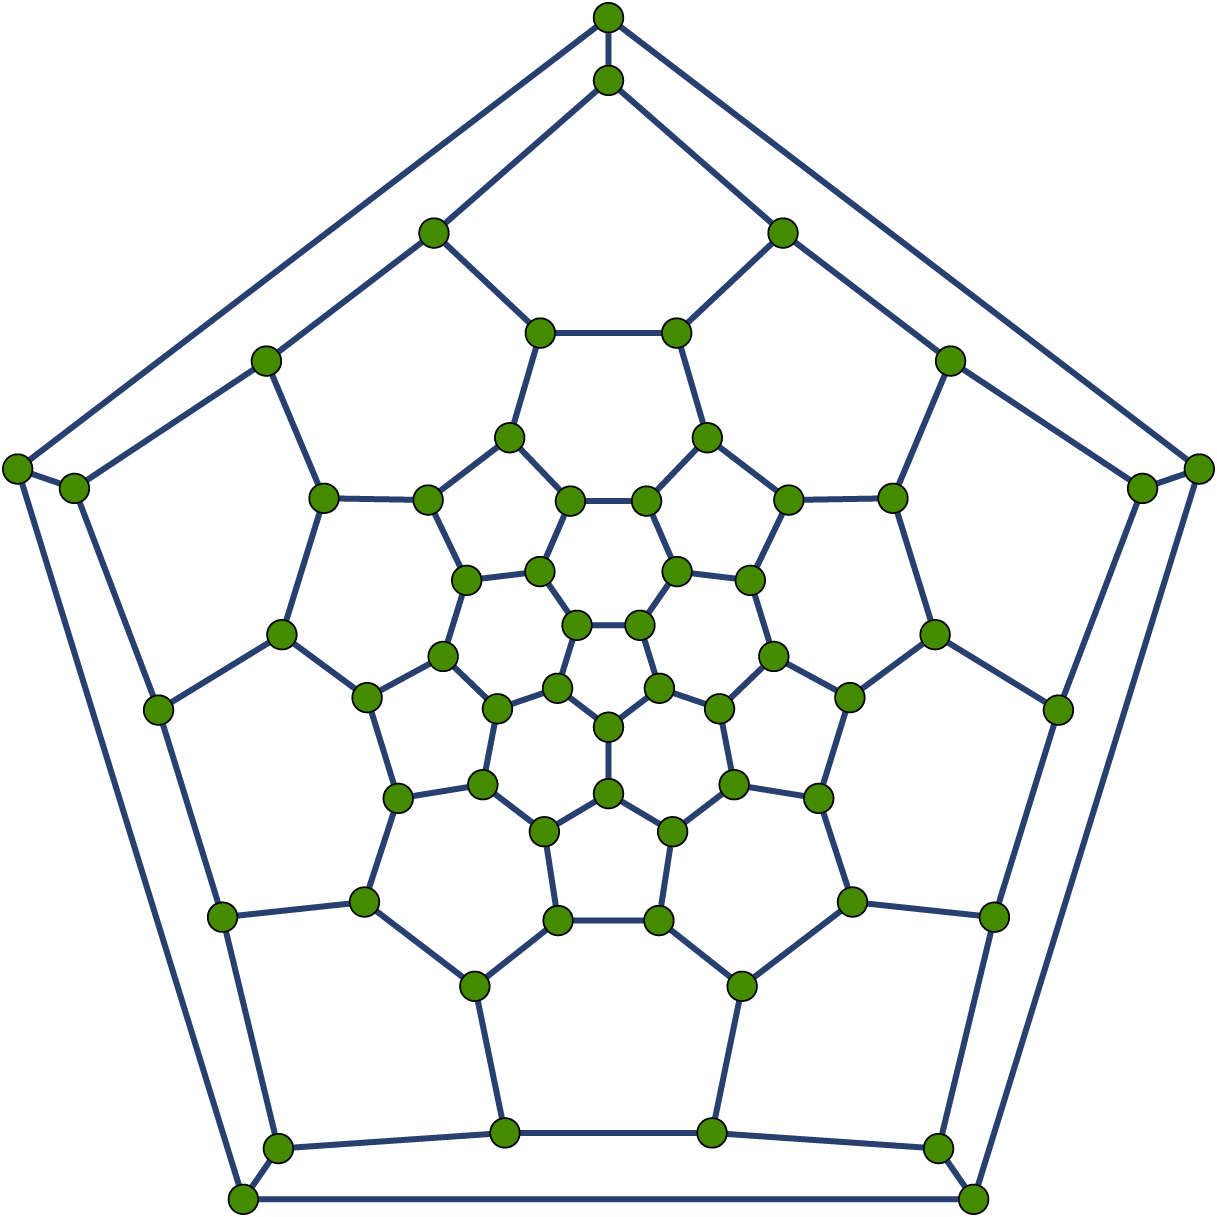
\includegraphics[width=0.22\textwidth]{Graph1.png}
		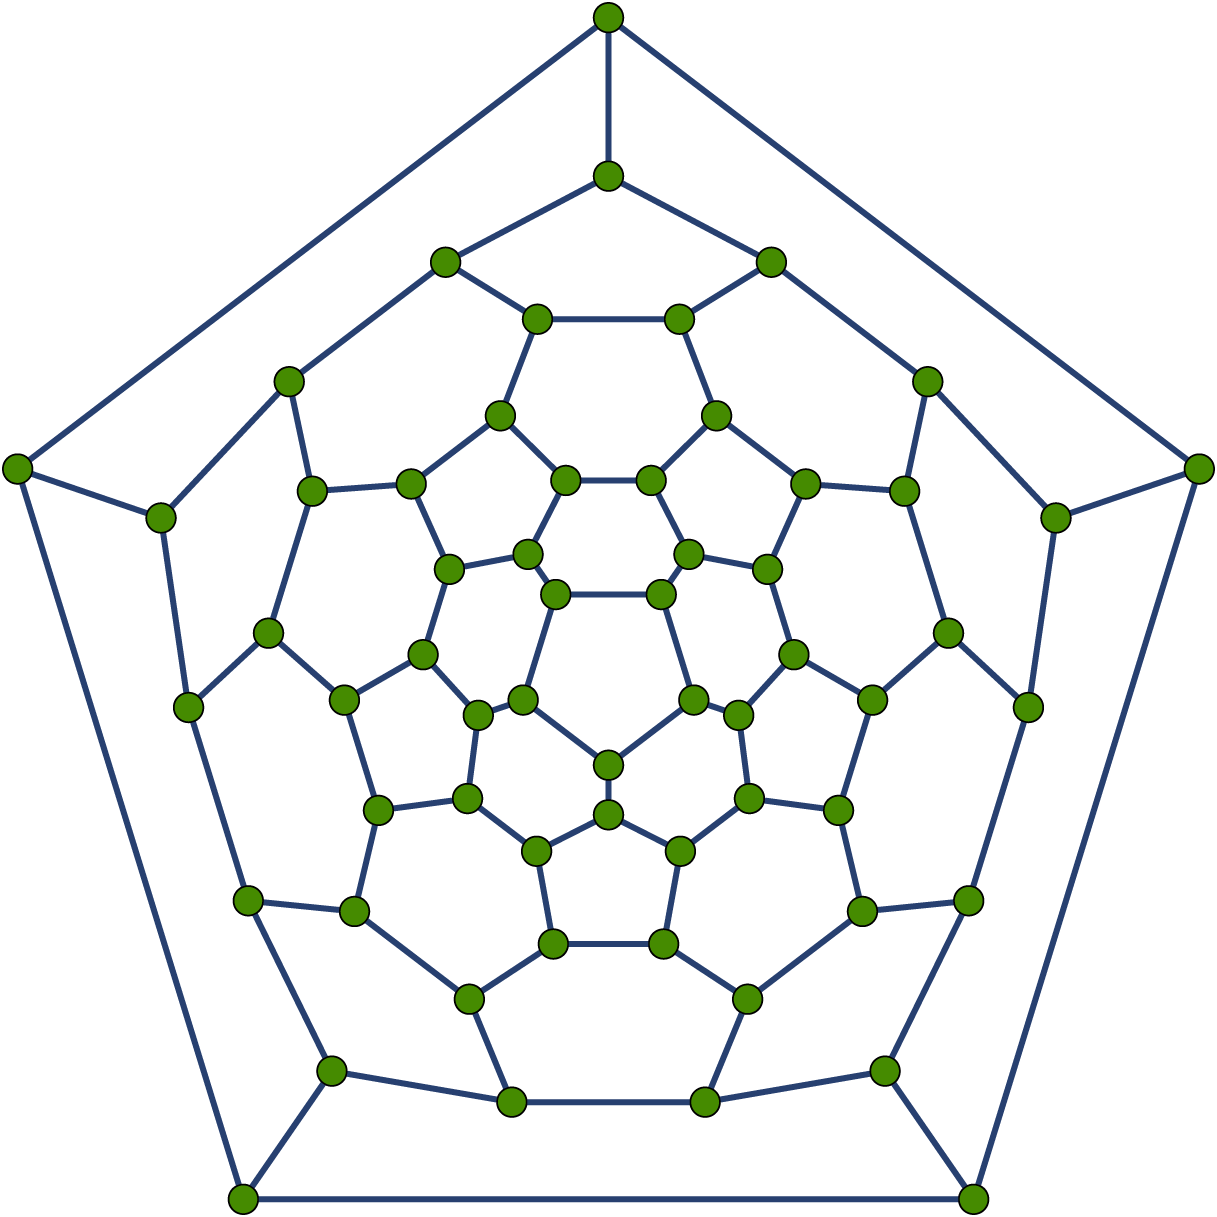
\includegraphics[width=0.22\textwidth]{Graph2.png}
		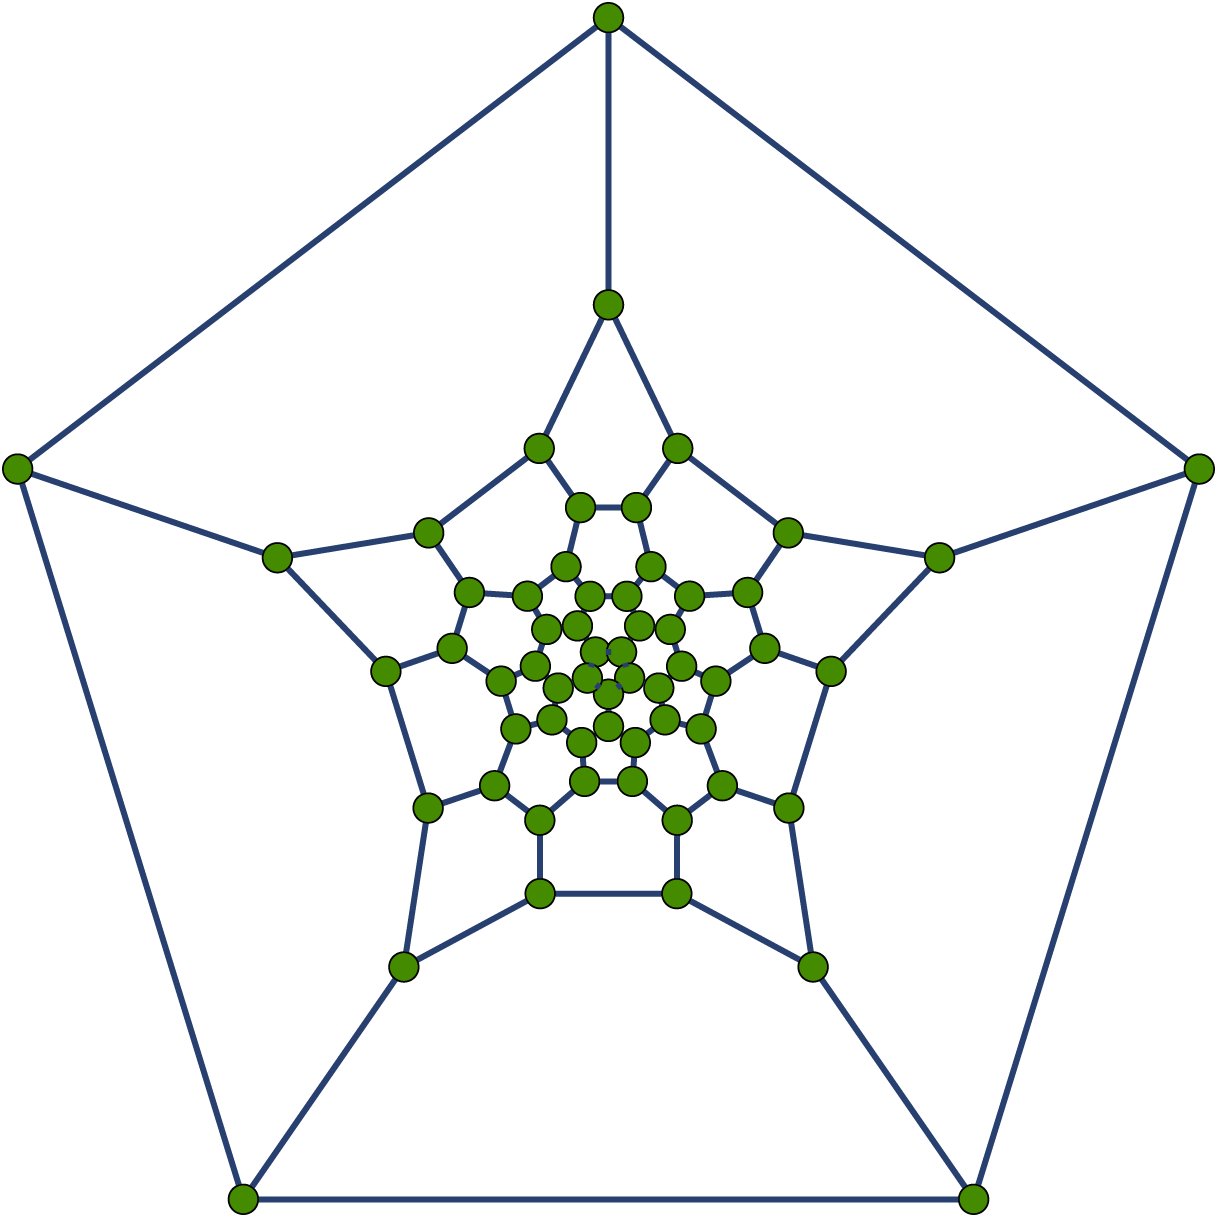
\includegraphics[width=0.22\textwidth]{Graph3.png}
		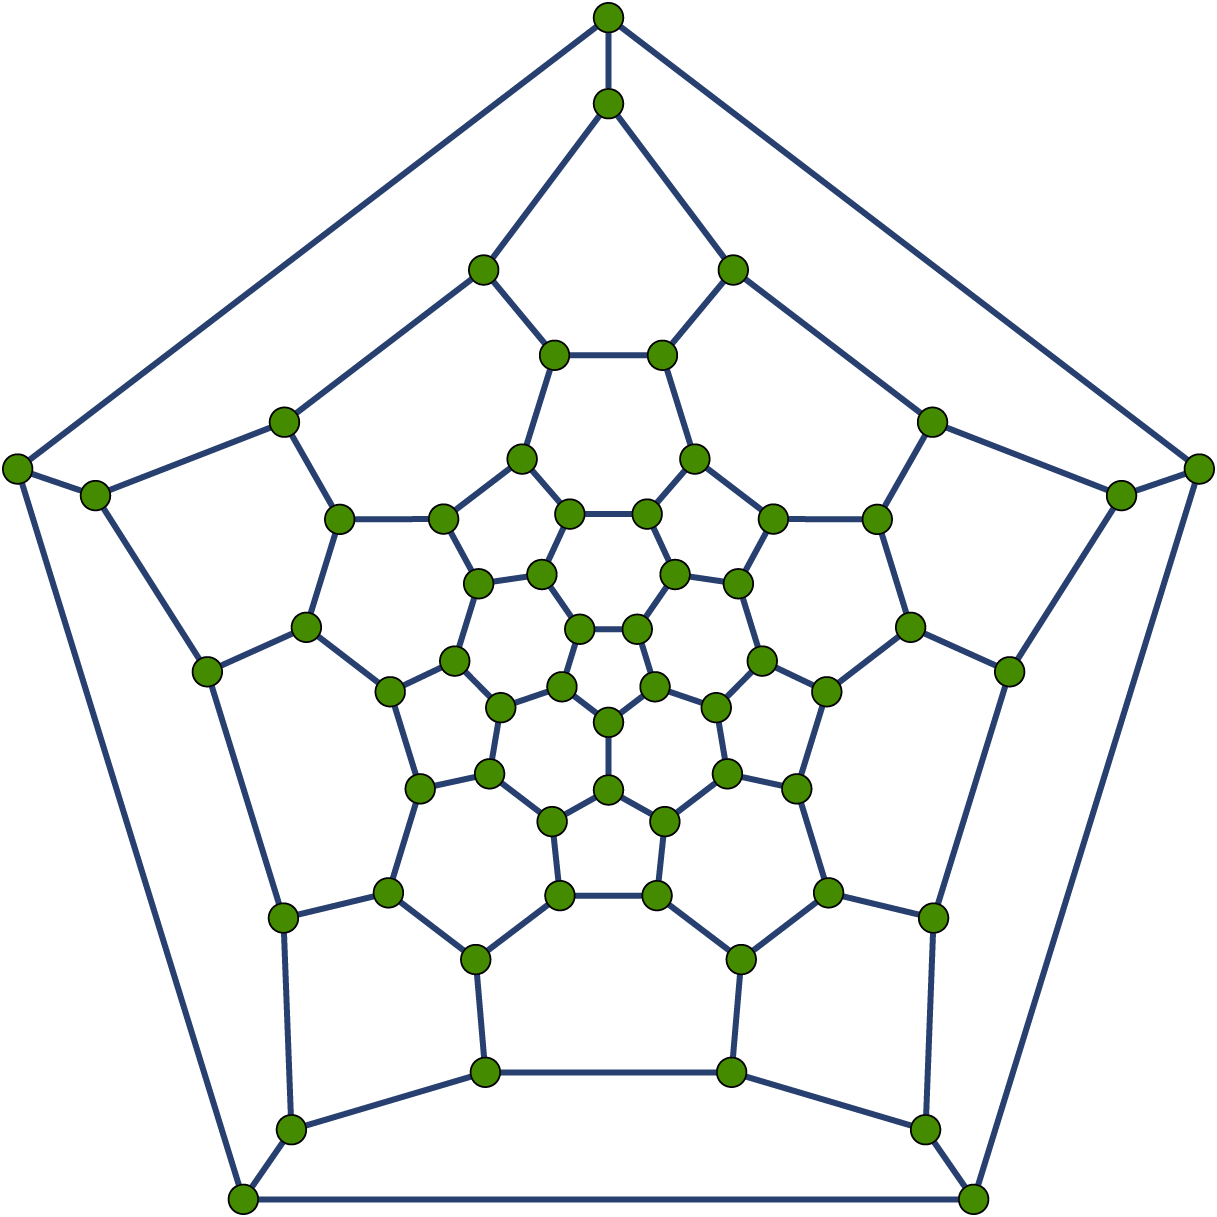
\includegraphics[width=0.22\textwidth]{Graph4.png}
		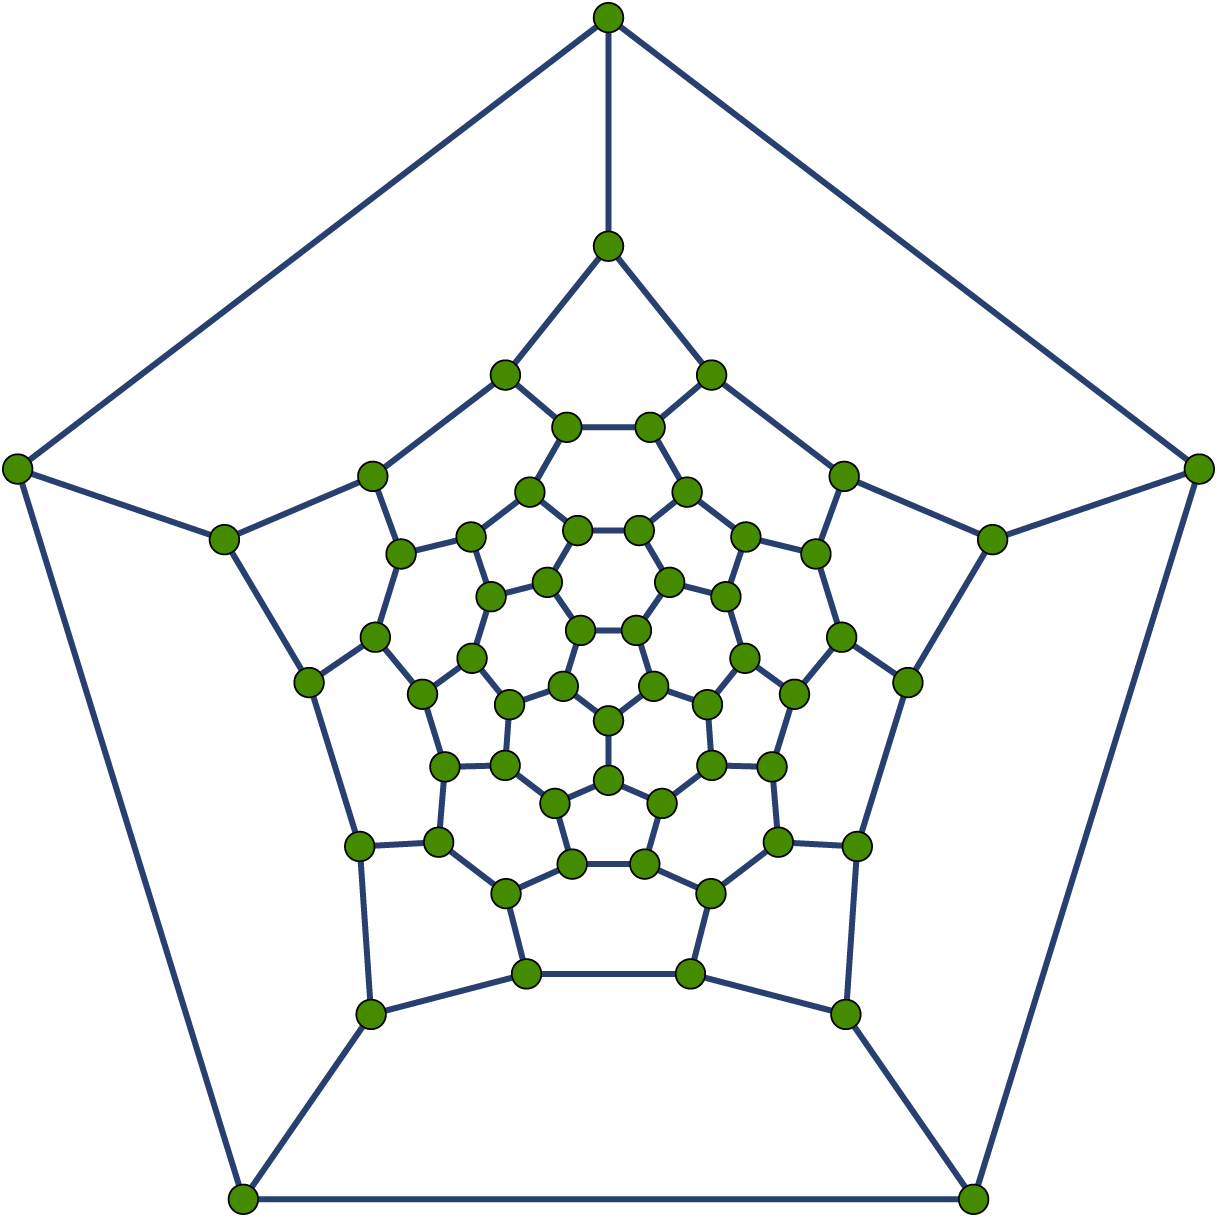
\includegraphics[width=0.22\textwidth]{Graph5.png}
		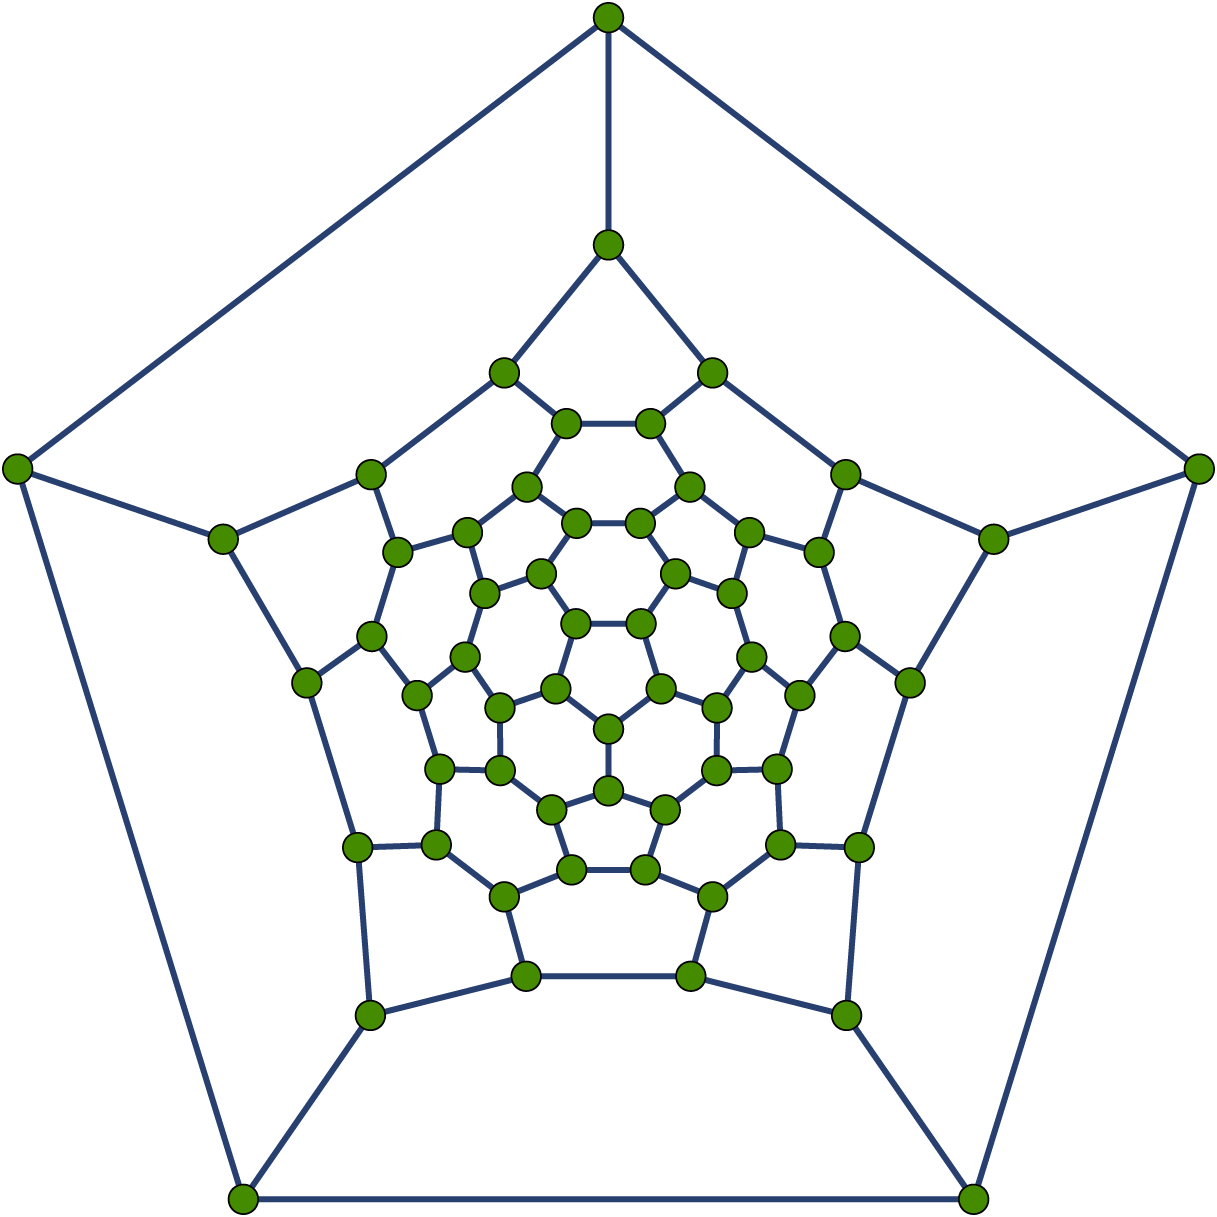
\includegraphics[width=0.22\textwidth]{Graph6.png}
		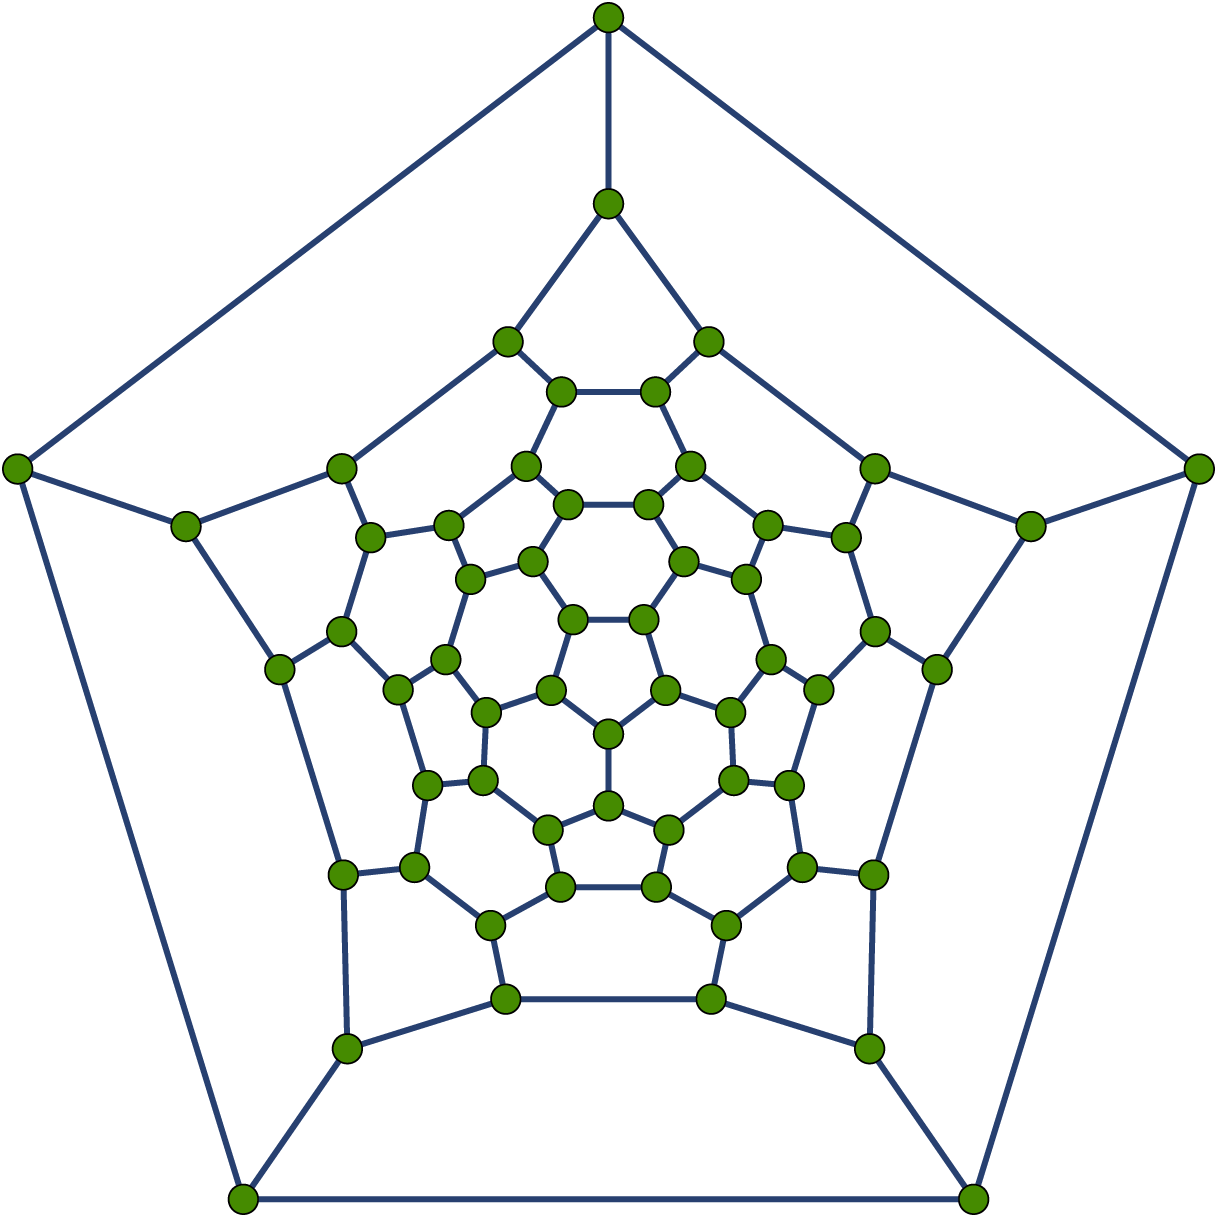
\includegraphics[width=0.22\textwidth]{Graph7.png}
		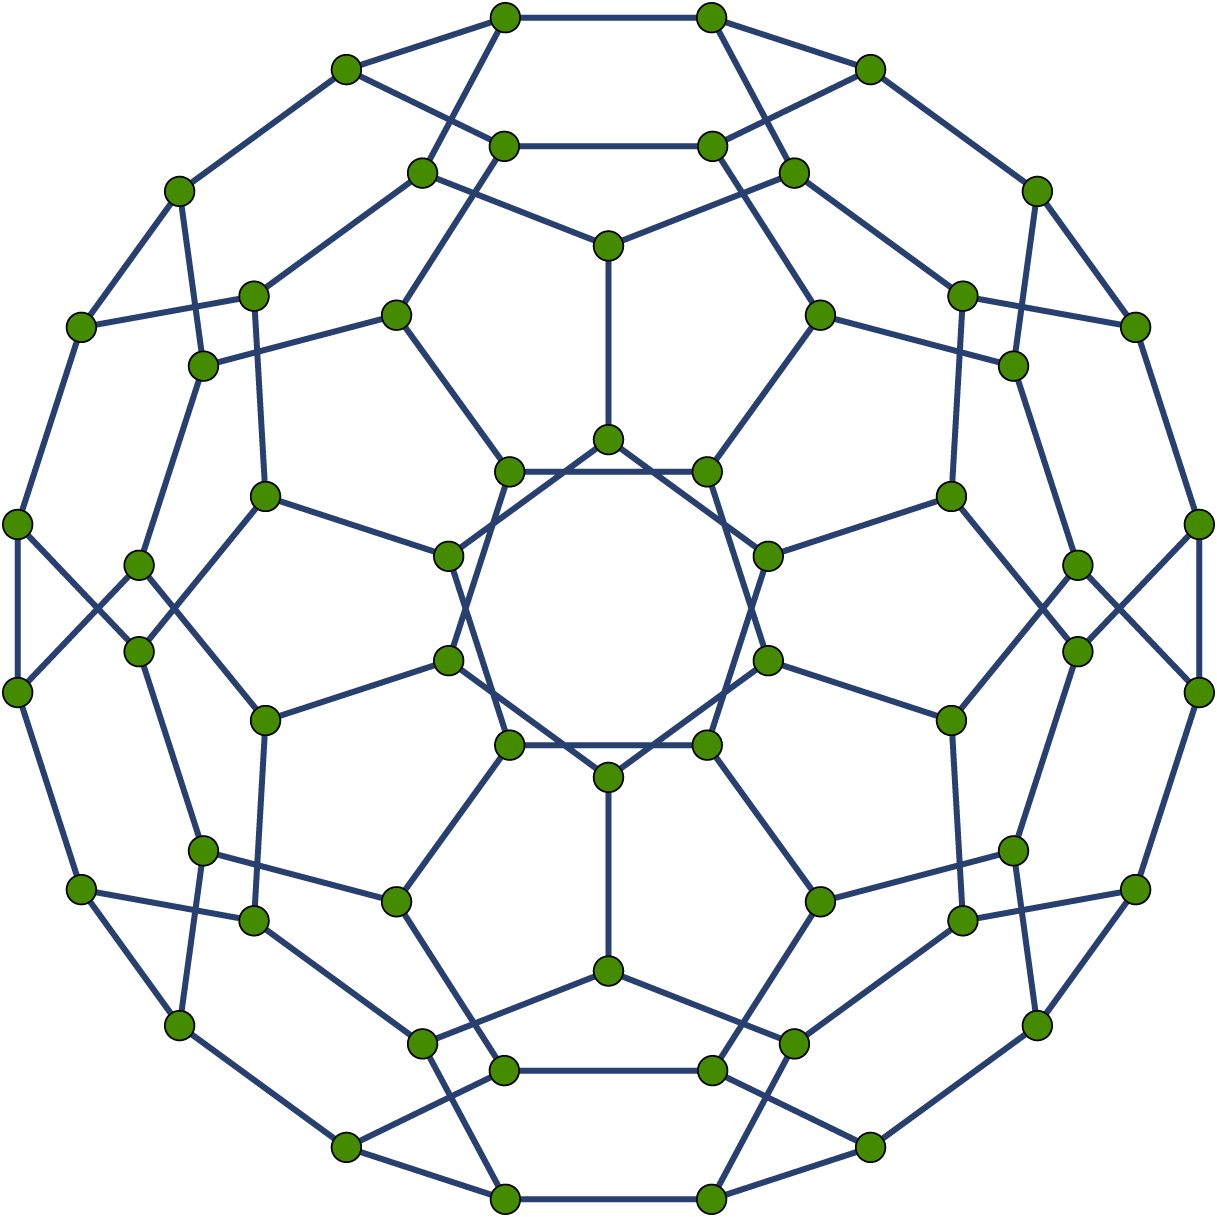
\includegraphics[width=0.22\textwidth]{Graph8.png}
        \label{pic:Graph2D}
        \caption{From the left to right: 2D fullerene structures created using {\bf ISchlegel}=1 to 8.}
 \end{figure}
              
%Fullerene Isomer Database
\section{Fullerene Isomer Database}
A database is provided for general isomers up to \C{100} and for IPR isomers up to
\C{120} including the number of Hamiltonian cycles. The database can be copied into
the main program folder and can be used to read the ring spiral pentagon indices.
The numbering scheme is identical to that the one chosen in the book by Fowler 
and Manolopoulus,\cite{Atlas}, that is each isomer in the book's appendix can be 
constructed easily from the database. An example is given in the input file   
{\it database.inp}.  The datafiles are formatted and can easily be read. It is our 
intention to extend the isomer list beyond \C{100}/\C{120} (without Hamiltonian cycles). 
New lists will be available on our website in time.  The determination of the number of
distinct Hamiltonian cycles is NP-complete and beyond 100 (120 for IPR) 
computationally too demanding. The longest file for our database ran for 3~months on a single 2.4 GHz AMD processor.
The directory database needs to be in the same directory as ``source'' or ``libgraph''.

%\clearpage


%References
\section{References}
\begin{thebibliography}{99}

\bibitem{Brinkmanx} G. Brinkmann, O. D. Friedrichs, A. Dress, and T. Harmuth, ``CaGe -- a virtual environment for studying some special classes of large molecules'', {\it Match-Commun. Math. Comput. Chem.} 233 (1997).
 
\bibitem{Brinkman} G. Brinkmann, ``Program Fullgen - a program for generating nonisomorphic fullerenes'', see http://cs.anu.edu.au/~bdm/plantri/.
 
\bibitem{Goedgebeur} G. Brinkmann, J. Goedgebeur, B. McKay, ``Program Buckygen - a program for the efficient generation of all nonisomorphic fullerenes'',
see http://caagt.ugent.be/buckygen/.

\bibitem{Pisanski} T. Pisanski, ``Program VEGA - A Mathematica based system for manipulating graphs'', see http://www.ijp.si/.

\bibitem{Tutte} W. T. Tutte, ``How to Draw a Graph'', {\it Proc. London Math. Soc.} {\bf 13}, 743�767 (1963).

\bibitem{Atlas} P. W. Fowler and D. E. Manolopoulus, ``An Atlas of Fullerenes'' (Dover Publ., New York, 2006).
 
\bibitem{Endo92} M. Endo and H.W. Kroto, ``Formation of carbon nanofibers'', {\it J. Phys. Chem.} {\bf 96}, 6941-6944 (1992).

\bibitem{Yoshida97} M. Yoshida, P. Fowler, {\it Chem. Phys. Lett.} {\bf 278}, 256�261(1997).

\bibitem{WS} L. Wirz, J. Avery, P. Schwerdtfeger, to be published.

\bibitem{Stone86} A. J. Stone and D. J. Wales, ``Formation of carbon nanofibers'', {\it Chem. Phys. Lett.} {\bf 128}, 501-503 (1986).

\bibitem{NumRec} W. T. Vetterling, B. P. Flannery, in ``Numerical Recipes in C - The Art of Scientific Computing'', chapter 10, section 6: Conjugate Gradient Methods in Multidimensions; W. H. Press, S. A. Teukolsky (Editors), , Cambridge University Press; 2nd edition (1992).

\bibitem{Wu87} Z. C. Wu, D. A. Jelski, and T. F. George, ``Vibrational Motions of
Buckminsterfullerene'', {\it Chem. Phys. Lett.} {\bf 137}, 291-295 (1987).

\bibitem{Plestenjak} B. Plestenjak, ``An algorithm for drawing Schlegel diagrams'', see http://www-lp.fmf.uni-lj.si/plestenjak/Papers/NICEGR.pdf.

\bibitem{Cioslowski2000} J. Cioslowski, N. Rao, D. Moncrieff, ``Standard Enthalpies of Formation of Fullerenes and Their
Dependence on Structural Motifs'', {\it J. Am. Chem. Soc.} {\bf 122}, 8265�8270 (2000).

\bibitem{Babic1995} D. Babi\'c, O. Ori, ``Matching polynomial and topological resonance energy of \C{70}'', {\it Chem. Phys. Lett.} {\bf 234}, 240-244 (1995).

\bibitem{Babic1997} D. Babi\'c, ``Topological Resonance Energy of Fullerenes'', {\it J. Chem. Inf. Comput. Sci.} {\bf 37}, 920-923 (1997).

\bibitem{Alcami} M. Alcam\'i, G. Sanchez, S. Diaz-Tendero, Y. Wang, F. Martin, ``Structural Patterns in Fullerenes Showing
Adjacent Pentagons: \C{20} to \C{72}'', {\it J. Nanosci. Nanotech.} {\bf 7}, 1329-1338 (2007).

\bibitem{HouseofGraphs} The House of Graphs website is at https://hog.grinvin.org/Fullerenes.

\bibitem{CYLview} C. Y. Legault, ``Program CYLview'', Universit\'e de Sherbrook, Canada. See http://www.cylview.org.

\bibitem{Avogadro} Program Avogadro, ``An advanced molecule editor and visualizer designed for cross-platform use in computational chemistry, molecular modeling, bioinformatics, materials science, and related areas'', see http://avogadro.openmolecules.net.

\bibitem{JMol} Program JyMOL, ``A Java-based development component'', see http://jmol.sourceforge.net/.

\bibitem{Pymol} Program Pymol, ``A user-sponsored molecular visualization system on an open-source foundation'', see http://www.pymol.org/.

\bibitem{vmd} Program VMD, ``Visual Molecular Dynamics'', http://www.ks.uiuc.edu/Research/vmd/.

\bibitem{Gabriel2008} A. T. Gabriel, T. Meyer, and G. Germano, 
``Molecular graphics of convex body fluids'', {\it J. Chem. Theory Comput.}
{\bf 4}, 468--476 (2008). The program is available at http://qmga.sourceforge.net/.

\bibitem{PSJA} P. Schwerdtfeger and J. Avery, ``Topological and Graph Theoretical Properties of Regular Fullerenes'', in preparation.

\bibitem{cvetkovic2002} D. Cvetkovi\'c, P. Fowler, P. Rowlinson, and D. Stevanovi�c, ``Constructing fullerene graphs from eigenvalues and angles'',
{\it Linear Algebra Appl.} {\bf 356}, 37�56 (2002).

\bibitem{Babic1995a} D. Babi\'c, ``Nomenclature and Coding of Fullerenes'', {\it J. Chem. Inf. Comput. Sci.} {\bf 35}, 515-526 (1995).

\bibitem{PSAJDB} P. Schwerdtfeger, D. Babi\'c, and J. Avery, ``Hamiltonian cycles in regular fullerenes'', in preparation.

\bibitem{NumericalRecipes} ``Numerical Recipes in Fortran 77. The Art of Scientific Computing'' (2nd Edition, 1992); see http://www.nr.com/.

\bibitem{Diaz} S. D\'iaz-Tendero, F. Mart\'in, and M. Alcam\'i, {\it ChemPhysChem} {\bf 6}, 92-100 (2005).

\bibitem{Fowler2000} P. W. Fowler, T. Heine, F. Zerbetto, {\it J. Phys. Chem.} {\bf 104}, 9625-9629 (2000).

\bibitem{Yildirim08} E. A. Yildirim, ``Two Algorithms for the Minimum Enclosing Ball Problem'', 
{\it SIAM Journal on Optimization}, {\bf 19}, 1368-1391 (2008) 

\bibitem{Hopp96} T. H. Hopp and C. P. Reeve, ``An Algorithm for Computing the Minimum Covering Sphere in Any Dimension'', 
NIST, US Department of Commerce (1996).

\bibitem{Heiney91} P. A. Heiney. J. E. Fischer, A. R. McGhie, W. J. Romanow, A. M. Denenstein, J. P. McCauley Jr., A. B. Smith, and D. E. Cox,
``Orientational ordering transition in solid \C{60}'', {\it Phys. Rev. Lett.} {\bf 66}, 2911-2914 (1991).

\bibitem{pisanski95} T. Pisanski, B. Plestenjak, and A. Graovac, ``Nice Program and its Application, {\it Croat. Chem. Acta} {\bf 68}, 283�292 (1995).

\bibitem{Ceulemans} A. Ceulemans, B. C. Titeca, L. F. Chibotaru, I. Vos, and P. W. Fowler, ``Complete bond force fields for trivalent and deltahedral cages: Group theory and applications to cubane, closo-dodecaborane, and buckminsterfullerene'', {\it J. Phys. Chem. A} {\bf 105}, 8284-8295 (2001).

\bibitem{Hands04} I. D. Hands, J. L. Dunn, and C. A. Bates, ``A complete nearest-neighbor force field model for \C{60}'', 
{\it J. Chem. Phys.} {\bf 120}, 6912-6921 (2004).

\end{thebibliography}

\end{document}

